% !TEX program = pdflatex
\documentclass[10pt]{article}

% ---------- PACKAGES ----------
\usepackage[margin=1in]{geometry}
\usepackage[T1]{fontenc}
\usepackage{lmodern}
\usepackage{setspace}
\usepackage{amsmath, amssymb}

\usepackage{xcolor}
\definecolor{softpink}{rgb}{0.99, 0.74, 0.71}

\usepackage{tikz}
\usetikzlibrary{shapes,patterns}

\usepackage{enumitem}
\usepackage[normalem]{ulem}
\usepackage{float}

\usepackage[hidelinks]{hyperref}
\usepackage{tocloft}

\usepackage[most]{tcolorbox}
\usepackage[table]{xcolor}


% ---------- GRAPH SYSTEM (pgfplots + cue + candycolors) ----------
\usepackage{pgfplots}
\pgfplotsset{compat=1.18}

% ---------- BABY CANDY COLORS ----------
\definecolor{babyblue}{rgb}{0.68, 0.85, 0.90}
\definecolor{babypink}{rgb}{1.00, 0.80, 0.86}
\definecolor{babyyellow}{rgb}{1.00, 0.95, 0.70}
\definecolor{babyorange}{rgb}{1.00, 0.82, 0.65}
\definecolor{babygreen}{rgb}{0.75, 0.90, 0.75}


\pgfplotsset{
    candycolors/.style={
        ybar,
        bar width=18pt,
        draw=black,
        fill=softpink!60,
        axis lines=left,
        tick style={black},
        label style={black},
        title style={black,font=\bfseries},
        major grid style={dashed,gray!30},
        ymajorgrids=true,
        xmajorgrids=false
    }
}
\pgfplotsset{
    candycycle/.style={
        cycle list={
            {fill=babyblue,   draw=black},
            {fill=babypink,   draw=black},
            {fill=babyyellow, draw=black},
            {fill=babyorange, draw=black},
            {fill=babygreen,  draw=black}
        }
    }
}


\newcommand{\cue}[2][]{%
\begin{tikzpicture}
\begin{axis}[
    candycolors,
    width=0.9\textwidth,
    height=6cm,
    enlargelimits=false,
    ymin=0,
    #1
]
#2
\end{axis}
\end{tikzpicture}
}

\setlength{\parindent}{0pt}
\setlength{\parskip}{0.35em}

\onehalfspacing

\begin{document}

\begin{titlepage}
\centering

\vspace*{1cm}

{\LARGE MIE Lecture Notes}\\[0.4cm]
{\large Probability and Statistics}\\[0.4cm]
{\large Cheryl Shi}\\[1cm]
{\large Contents}

\vspace{1cm}

\noindent
\textbf{Chapter 1: Probability Foundations}
\dotfill
\hyperref[chap:one]{\pageref*{chap:one}}

\vspace{0.3cm}

\noindent\hspace{0.5cm}
1.1 Sampling Methods
\dotfill
\hyperref[sec:sampling]{\pageref*{sec:sampling}}

\noindent\hspace{0.5cm}
1.2 Data, Variables, and Distributions
\dotfill
\hyperref[sec:data_variables]{\pageref*{sec:data_variables}}

\noindent\hspace{0.5cm}
1.3 Graphical Representations of Data
\dotfill
\hyperref[sec:plots]{\pageref*{sec:plots}}

\vspace{0.6cm}

\noindent
\textbf{Chapter 2: Random Variables and Distributions}
\dotfill
\hyperref[chap:two]{\pageref*{chap:two}}

\vspace{0.3cm}

\noindent\hspace{0.5cm}
2.1 Experiments, Sample Spaces, and Events
\dotfill
\hyperref[sec:sample_space_events]{\pageref*{sec:sample_space_events}}

\noindent\hspace{0.5cm}
2.2 Event Operations and Probability Rules
\dotfill
\hyperref[sec:event_probability]{\pageref*{sec:event_probability}}

\noindent\hspace{0.5cm}
2.3 Counting Techniques and Equally Likely Outcomes
\dotfill
\hyperref[sec:counting]{\pageref*{sec:counting}}

\noindent\hspace{0.5cm}
2.4 Conditional Probability and Independence
\dotfill
\hyperref[sec:conditional]{\pageref*{sec:conditional}}

\vspace{0.6cm}

\noindent
\textbf{Chapter 3: Statistical Inference}
\dotfill
\hyperref[chap:three]{\pageref*{chap:three}}

\vspace{0.3cm}

\noindent\hspace{0.5cm}
3.1 Random Variables and Their Interpretation
\dotfill
\hyperref[sec:rv_definition]{\pageref*{sec:rv_definition}}

\noindent\hspace{0.5cm}
3.2 Discrete Random Variables
\dotfill
\hyperref[sec:rv_types]{\pageref*{sec:rv_types}}

\noindent\hspace{0.5cm}
3.3 Probability Mass Functions
\dotfill
\hyperref[sec:pmf]{\pageref*{sec:pmf}}

\noindent\hspace{1.2cm}
3.3.1 PMFs for Discrete Random Variables
\dotfill
\hyperref[sec:pmf_discrete]{\pageref*{sec:pmf_discrete}}

\noindent\hspace{0.5cm}
3.4 Cumulative Distribution Function (CDF)
\dotfill
\hyperref[sec:cdf]{\pageref*{sec:cdf}}

\noindent\hspace{1.2cm}
3.4.1 CDF for Discrete Random Variables
\dotfill
\hyperref[sec:cdf_discrete]{\pageref*{sec:cdf_discrete}}

\noindent\hspace{1.2cm}
3.4.2 CDF for Continuous Random Variables
\dotfill
\hyperref[sec:cdf_continuous]{\pageref*{sec:cdf_continuous}}

\noindent\hspace{0.5cm}
3.5 Continuous Sample Space and Continuous Random Variables
\dotfill
\hyperref[sec:continuous_rv]{\pageref*{sec:continuous_rv}}

\noindent\hspace{0.5cm}
3.6 Probability Density Function (PDF)
\dotfill
\hyperref[sec:pdf]{\pageref*{sec:pdf}}

\noindent\hspace{0.5cm}
3.7 Joint Probability Distributions
\dotfill
\hyperref[sec:joint]{\pageref*{sec:joint}}

\noindent\hspace{1.2cm}
3.7.1 Joint Distributions for Discrete Random Variables
\dotfill
\hyperref[sec:joint_discrete]{\pageref*{sec:joint_discrete}}

\noindent\hspace{1.2cm}
3.7.2 Joint Distributions for Continuous Random Variables
\dotfill
\hyperref[sec:joint_continuous]{\pageref*{sec:joint_continuous}}

\noindent\hspace{0.5cm}
3.8 Marginal Distributions
\dotfill
\hyperref[sec:marginal]{\pageref*{sec:marginal}}

\noindent\hspace{0.5cm}
3.9 Conditional Distributions
\dotfill
\hyperref[sec:conditional]{\pageref*{sec:conditional}}

\noindent\hspace{0.5cm}
3.10 Independence
\dotfill
\hyperref[sec:independence]{\pageref*{sec:independence}}

\end{titlepage}

\newpage


\section*{Chapter 1}
\label{chap:one}


\subsection*{Statistics Definitions}


\textbf{Global definition:} Statistics involves collecting, organizing, summarizing, presenting, and analyzing data, as well as making inferences, conclusions, and decisions based on data.

\textbf{Statistical definition:} A \underline{statistic} is a numerical value calculated from data (e.g.\ mean, proportion, standard deviation).

\vspace{0.5em}

\begin{center}
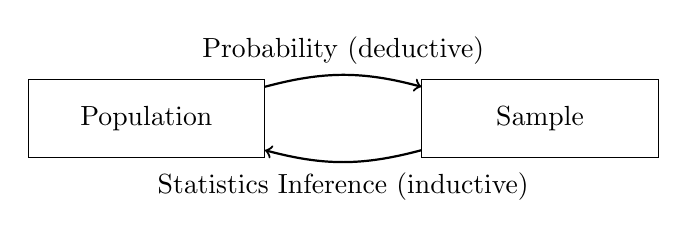
\begin{tikzpicture}[
    box/.style={draw, rectangle, minimum width=3cm, minimum height=1cm},
    arrow/.style={->, thick}
]

\node[box] (pop) at (0,0) {Population};
\node[box] (samp) at (5,0) {Sample};

% top line
\draw[arrow] (pop) to[bend left=15] node[above] {Probability (deductive)} (samp);

% bottom line
\draw[arrow] (samp) to[bend left=15] node[below] {Statistics Inference (inductive)} (pop);

\end{tikzpicture}
\end{center}


\subsection*{Basic Terminology}
\underline{Individuals}: Objects on which data are collected (people, animals, plots of land, etc.).\\
\underline{Variable}: Any characteristic of an individual.\\
\underline{Population}: The entire group of individuals of interest.\\
\underline{Sample}: A subset of individuals taken from the population.\\
\underline{Statistical Inference}: Drawing conclusions about a population based on a sample.

\section*{Sampling Methods}
\label{sec:sampling}


\underline{Simple Random Sample (SRS):}
\begin{itemize}
  \item Every possible group of size $n$ has an equal chance of being selected.
  \item Helps avoid bias in sampling.
  \item Can be selected using random number tables or software.
\end{itemize}

\underline{Stratified Random Sampling:}
\begin{itemize}
  \item The population is divided into \underline{homogeneous groups} 
        \textit{(individuals are similar with respect to the variable being studied)} 
        called \underline{strata}.
  \item A simple random sample is taken from each \underline{stratum}. 
        \textit{(one subgroup of the population created)}
  \item Ensures that important subgroups are neither over nor under represented.
\end{itemize}

\section*{Data, Variables, and Distributions}
\label{sec:data_variables}

\subsection*{Types of Variables}

\underline{Categorical Variable}: Places individuals into categories (e.g.\ gender, major). These are qualitative.

\underline{Quantitative Variable}: Takes numerical values for which arithmetic operations are meaningful.

\begin{itemize}
    \item \underline{Discrete}
    \item \underline{Continuous}
\end{itemize}


\subsection*{Distributions}

\underline{Distribution}: Describes what values a variable takes and how often those values occur.
When examining a distribution, look for:
\begin{itemize}
    \item \textbf{Shape}
    \item \textbf{Center}
    \item \textbf{Spread}
    \item \textbf{Outliers}
\end{itemize}
\underline{Outlier}: An individual value that falls outside the overall pattern of the data.

\subsection*{Describing Distributions with Numbers}

\underline{Central Tendency}: Describes where the data cluster or center.

\underline{Central Tendency}: Describes where the data cluster or center.
\begin{itemize}
    \item \underline{Mean}: average value
    \item \underline{Median}: middle value
\end{itemize}

\bigskip

\noindent
\underline{Mean (Arithmetic Mean):}
\[
\boxed{
\bar{x} = \frac{1}{n}\sum_{i=1}^{n} x_i
}
\]

\bigskip

\noindent
\underline{Median:}
\[
\boxed{
\tilde{x} =
\begin{cases}
x_{\left(\frac{n+1}{2}\right)}, & \text{if } n \text{ is odd} \\[6pt]
\displaystyle \frac{x_{\left(\frac{n}{2}\right)} + x_{\left(\frac{n}{2}+1\right)}}{2}, & \text{if } n \text{ is even}
\end{cases}
}
\]

\bigskip

\begin{center}
\begin{tcolorbox}[
    colback=softpink!3,
    colframe=softpink!70!black,
    colbacktitle=softpink,
    coltitle=black,
    fonttitle=\bfseries,
    title=Theorem 1.1,
    width=0.9\textwidth
]
\begin{enumerate}
    \item The mean is more sensitive to extreme values than the median.
    \item Changing a single data value will always change the mean, but may not change the median.
    \item If a distribution is exactly symmetric, the mean and median are equal.
\end{enumerate}
\end{tcolorbox}
\end{center}

\bigskip


\noindent
\underline{Trimmed Mean:}  
The mean computed after removing extreme values.

\[
\boxed{
\bar{x}_{\text{trim}} = \frac{1}{n - 2k}
\sum_{i=k+1}^{n-k} x_{(i)}
}
\]

\noindent
where \(k\) values are removed from both ends of the ordered data. (normally given in question like 10\% )

\subsection*{Measures of Spread}

\underline{Range}:  
Maximum minus minimum. Very sensitive to extreme values.

\underline{Sample Variance}:  
Measures the average squared deviation from the mean.

\[
\boxed{
s^2 = \frac{1}{n-1} \sum_{i=1}^{n} (x_i - \bar{x})^2
}
\]

\underline{Standard Deviation}:  
The square root of the sample variance.

\[
\boxed{
s = \sqrt{s^2}
}
\]

\underline{Degrees of Freedom}:  
The number of independent pieces of information available to estimate variability.  
For sample variance: $df = n - 1$.

\section*{Graphical Representations of Data}
\label{sec:plots}

\underline{Scatter Plot}:  
Used to display the relationship between two quantitative variables $(x, y)$.  
A scatter plot helps identify trends, patterns, and associations between variables.

\underline{Stem-and-Leaf Plot}:  
An intermediate step between raw data and a frequency table.  
Preserves the original data values while showing the distribution.

\[
\begin{array}{c|c}
\text{Stem} & \text{Leaf} \\
\hline
1 & 2\;4\;7 \\
2 & 1\;3\;5\;8 \\
3 & 0\;4\;6
\end{array}
\]

\underline{Relative Frequency Table}:  
Shows the proportion of observations in each class.

\[
\begin{array}{c|c|c|c}
\text{Class Interval} & \text{Class Midpoint} & \text{Frequency} & \text{Relative Frequency} \\
\hline
10\text{--}19 & 14.5 & 3 & 0.30 \\
20\text{--}29 & 24.5 & 4 & 0.40 \\
30\text{--}39 & 34.5 & 3 & 0.30
\end{array}
\]

\underline{Histogram}:  
A graphical representation of a frequency or relative frequency table using contiguous bars.

When describing the shape of a histogram, we commonly classify it as:
\begin{itemize}
    \item \textbf{Symmetric}
    \item \textbf{Skewed right} (positively skewed)
    \item \textbf{Skewed left} (negatively skewed)
\end{itemize}

\begin{center}
\cue[
    candycycle,
    xlabel={Class},
    ylabel={Frequency},
    title={\textbf{Symmetric distribution example}},
    xmin=0.5, xmax=5.5,
    ymin=0, ymax=9,
    xtick={1,2,3,4,5},
    xticklabels={10--19,20--29,30--39,40--49,50--59},
    enlarge x limits=0.15
]{
    \addplot coordinates {(1,2)};
    \addplot coordinates {(2,5)};
    \addplot coordinates {(3,7)};
    \addplot coordinates {(4,5)};
    \addplot coordinates {(5,2)};

    % Smooth guide curve
    \addplot[smooth, thick, black]
        coordinates {(1,2) (2,5) (3,7) (4,5) (5,2)};
}
\end{center}



\section*{Chapter 2, Jan 9th}
\label{chap:two}

\section*{Experiments, Sample Spaces, and Events}
\label{sec:sample_space_events}

\underline{Experiment}: A process that generates an outcome.

\vspace{0.5em}

\underline{Sample Space ($S$)}: The set of all possible outcomes of an experiment.

\vspace{1em}

\textbf{Example 1:}

Select 3 items from a production line. Each item can be classified as either defective ($D$) or non-defective ($N$).

\[
S = \{ DDD, DDN, DND, NDD, DNN, NDN, NND, NNN \}
\]

Since each item has 2 possible outcomes,
\[
|S| = 2^3 = 8
\]

\vspace{1em}

\textbf{Example 2:}

\[
S = \{ (x,y) \mid x^2 + y^2 \le 4 \}
\]

\vspace{1em}

\underline{Event ($A$)}: A subset of the sample space $S$.

\vspace{0.5em}

\textbf{Examples of events:}
\[
A = \{ DDD, DDN, DND, NDD \}
\]
\[
B = \{ NNN \}
\]
\[
C = \{ (x,y) \mid x^2 + y^2 \le 4 \}
\]

\vspace{1em}

\section*{Event Operations and Probability Rules}
\label{sec:event_probability}

\underline{Event Operations}:
\begin{itemize}
  \item \underline{Complement}: $A^c$ (or $A'$)
  \item \underline{Intersection}: $A \cap B$
  \item \underline{Union}: $A \cup B$
  \item \underline{Null Event}: $\varnothing$
\end{itemize}

If
\[
A \cap B = \varnothing,
\]
then $A$ and $B$ are \underline{mutually exclusive}.

\vspace{1em}

\textbf{Example (Venn Diagram):}

\begin{center}
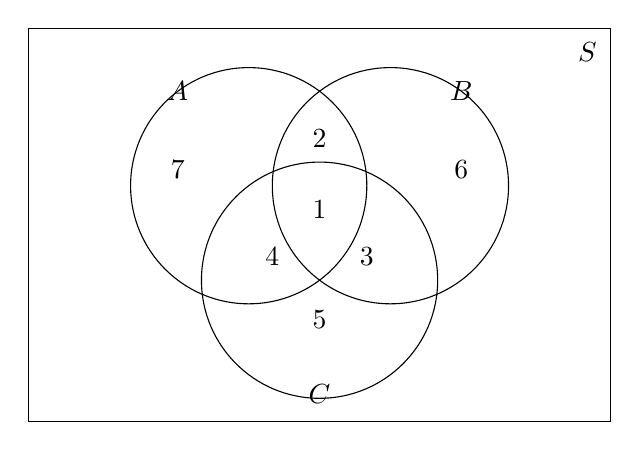
\begin{tikzpicture}[scale=1]

% Sample space
\draw (-2.8,-3) rectangle (4.6,2);

% Circles
\draw (0,0) circle (1.5);        % A
\draw (1.8,0) circle (1.5);      % B
\draw (0.9,-1.2) circle (1.5);   % C

% Labels
\node at (-0.9,1.2) {$A$};
\node at (2.7,1.2) {$B$};
\node at (0.9,-2.65) {$C$};
\node at (4.3,1.7) {$S$};

% Region numbers
\node at (-0.9,0.2) {7};        % A only
\node at (0.9,0.6) {2};         % A ∩ B
\node at (2.7,0.2) {6};         % B only
\node at (0.3,-0.9) {4};        % A ∩ C
\node at (1.5,-0.9) {3};        % B ∩ C
\node at (0.9,-0.3) {1};        % A ∩ B ∩ C
\node at (0.9,-1.7) {5};        % C only

\end{tikzpicture}
\end{center}

\[
A = \{ DDD, DDN, DND, NDD \}, \quad
B = \{ NNN \}
\]

\[
A \cup B = \{ DDD, DDN, DND, NDD, NNN \}
\]

\[
A \cap B = \varnothing
\]

\section*{Chapter 2: January 12}

\subsection*{Review}
{\itshape

\begin{enumerate}
    \item \underline{Experiment}: A process that generates an outcome.
    
    \item \underline{Sample Space} ($S$): The set of all possible outcomes of an experiment.
    
    \item \underline{Event Operations}:
    \begin{itemize}
        \item Complement: $A' \; (A^c)$
        \item Intersection: $A \cap B$
        \item Union: $A \cup B$
        \item Null Event: $\varnothing$
    \end{itemize}
    
    \item If $A \cap B = \varnothing$, then $A$ and $B$ are called \underline{mutually exclusive}.
\end{enumerate}

\fbox{
\parbox{0.95\textwidth}{
\[
(A \cap B)' = A' \cup B'
\]
\[
(A \cup B)' = A' \cap B'
\]
\[
A \cap \varnothing = \varnothing
\]
\[
A \cup \varnothing = A
\]
\[
A \cap (B \cup C) = (A \cap B) \cup (A \cap C)
\]
}}
}

\subsection*{Probability}

$P(A)$ = \underline{probability} of event $A$: the proportion of times the event occurs in infinitely many repetitions of the experiment.

\medskip

\begin{center}
\begin{tcolorbox}[
    colback=softpink!3,
    colframe=softpink!70!black,
    colbacktitle=softpink,
    coltitle=black,
    fonttitle=\bfseries,
    title=Theorem 2.1,
    width=0.9\textwidth
]
\[
0 \le P(A) \le 1
\]
\end{tcolorbox}
\end{center}

\medskip


\fbox{
\parbox{0.95\textwidth}{
\[
P(A) + P(A') = 1
\]

\[
P(A \cup B) = P(A) + P(B) - P(A \cap B)
\]

\[
\begin{aligned}
P(A \cup B \cup C) =\;& P(A) + P(B) + P(C) \\
&- P(A \cap B) - P(A \cap C) - P(B \cap C) \\
&+ P(A \cap B \cap C)
\end{aligned}
\]
}}

\medskip

\subsection*{Mutually Exclusive Events}

\underline{Definition}:  
If $A_1, A_2, \ldots, A_n$ are mutually exclusive, then
\[
P(A_1 \cup A_2 \cup \cdots \cup A_n)
=
P(A_1) + P(A_2) + \cdots + P(A_n)
\]

If
\[
A_1 \cup A_2 \cup \cdots \cup A_n = S,
\]
then $\{A_1, A_2, \ldots, A_n\}$ is a \underline{partition} of $S$.

\medskip
\begin{figure}[H]
\centering
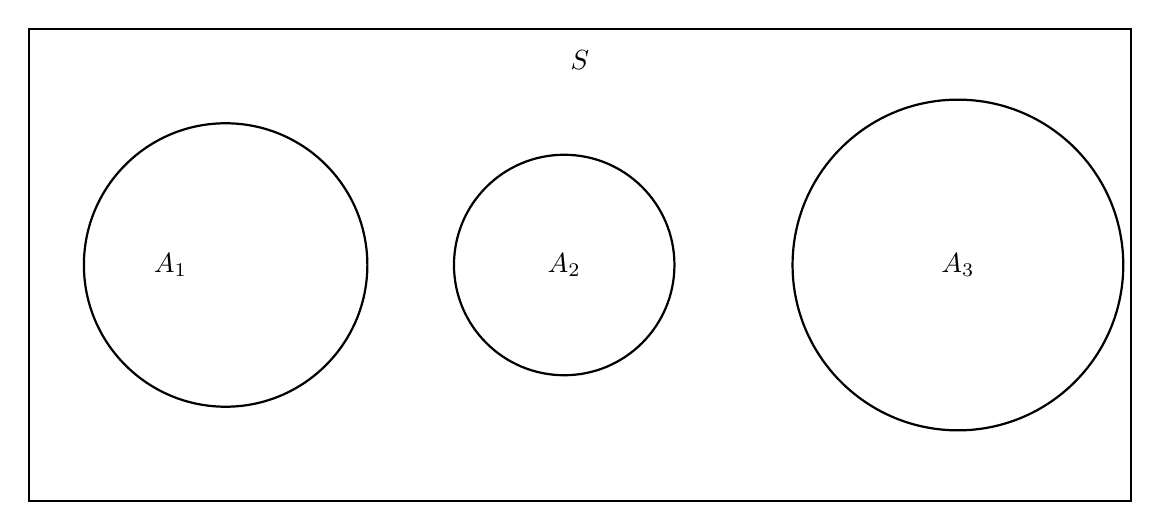
\begin{tikzpicture}[scale=1]

% Sample space
\draw[thick] (0,0) rectangle (14,6);
\node at (7,5.6) {$S$};

% A1
\draw[thick] (2.5,3) circle (1.8);
\node at (1.8,3) {$A_1$};

% A2
\draw[thick] (6.8,3) circle (1.4);
\node at (6.8,3) {$A_2$};

% A3
\draw[thick] (11.8,3) circle (2.1);
\node at (11.8,3) {$A_3$};

\end{tikzpicture}
\caption{Partition of the sample space $S$ into $A_1, A_2, A_3$}
\end{figure}


\subsection*{Example}

In a class of 33 students:
\begin{itemize}
    \item 17 earned an A on the midterm
    \item 14 earned an A on the final
    \item 11 earned no A on either exam
\end{itemize}

Find the probability that a randomly selected student earned A's on \underline{both} exams.

\begin{figure}[H]
\centering
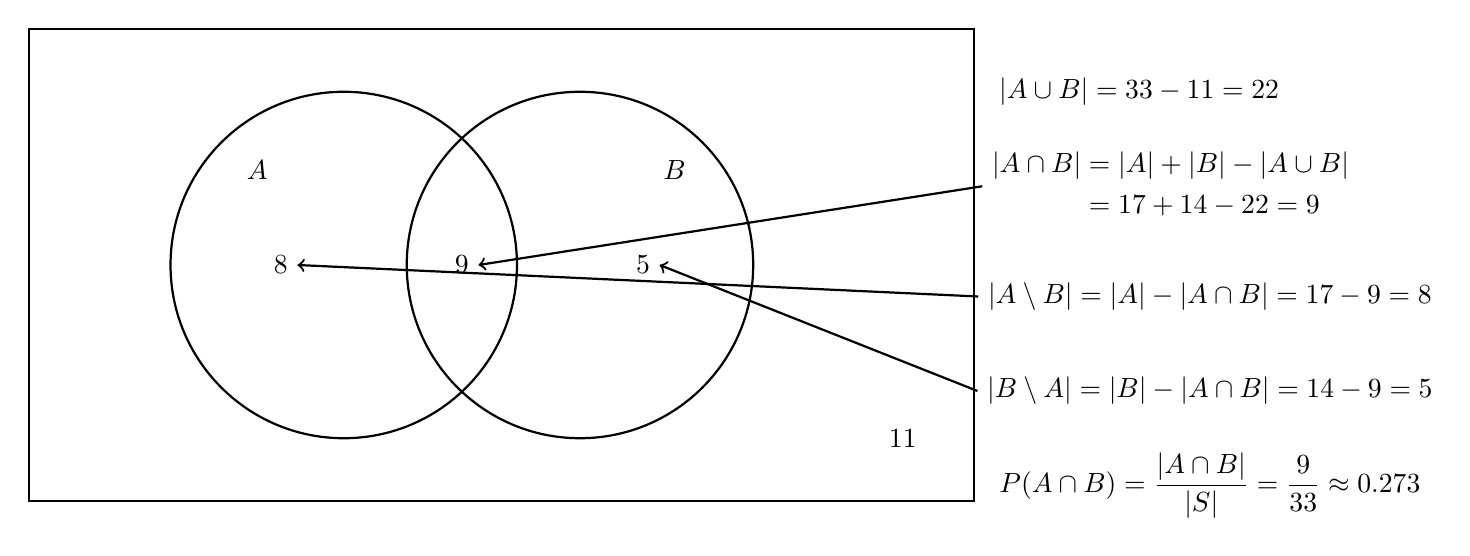
\begin{tikzpicture}[scale=1]

% -------------------------
% Sample space
% -------------------------
\draw[thick] (0,0) rectangle (12,6);

% -------------------------
% Circles A and B
% -------------------------
\draw[thick] (4,3) circle (2.2);
\draw[thick] (7,3) circle (2.2);

\node at (2.9,4.2) {$A$};
\node at (8.2,4.2) {$B$};

% -------------------------
% Region numbers
% -------------------------
\node (Aonly) at (3.2,3.0) {$8$};
\node (AB)    at (5.5,3.0) {$9$};
\node (Bonly) at (7.8,3.0) {$5$};
\node (outside) at (11.1,0.8) {$11$};

% -------------------------
% Calculation text blocks
% -------------------------
\node[align=left] (calcUnion) at (14.1 ,5.2) {$|A \cup B| = 33 - 11 = 22$};

\node[align=left] (calcInter) at (14.5,4.0) {$\begin{aligned}
|A \cap B|
&= |A| + |B| - |A \cup B| \\
&= 17 + 14 - 22 = 9
\end{aligned}$};

\node[align=left] (calcAonly) at (15,2.6) {$|A \setminus B| = |A| - |A \cap B| = 17 - 9 = 8$};

\node[align=left] (calcBonly) at (15,1.4) {$|B \setminus A| = |B| - |A \cap B| = 14 - 9 = 5$};

\node[align=left] (calcProb) at (15 ,0.2) {$P(A \cap B)=\dfrac{|A \cap B|}{|S|}=\dfrac{9}{33}\approx 0.273$};

% -------------------------
% Arrows pointing to regions
% -------------------------
\draw[->, thick] (calcInter.west) -- (AB.east);
\draw[->, thick] (calcAonly.west) -- (Aonly.east);
\draw[->, thick] (calcBonly.west) -- (Bonly.east);

\end{tikzpicture}
\caption{Events $A$: A on midterm, $B$: A on final, with region counts and calculations}
\end{figure}
\section*{Counting Techniques and Equally Likely Outcomes}
\label{sec:counting}


\medskip

\begin{center}
\begin{tcolorbox}[
    colback=softpink!5,
    colframe=softpink!70!black,
    colbacktitle=softpink,
    coltitle=black,
    fonttitle=\bfseries,
    title=Theorem 2.2 (Equally Likely Outcomes),
    width=0.9\textwidth
]
If the sample space \(S\) has a finite number of outcomes and all outcomes are equally likely, then for any event \(A\),
\[
P(A) = \frac{|A|}{|S|}.
\]

where
\[
|A| = \text{number of outcomes in event } A,
\qquad
|S| = \text{number of outcomes in the sample space}.
\]
\end{tcolorbox}
\end{center}

\medskip


\subsection*{Example 1: Poker Hands Basics}

A standard deck has:
\[
4 \text{ suits} \times 13 \text{ denominations (A,2,3,\ldots,Q,K)} = 52 \text{ cards}.
\]

A poker hand consists of 5 cards chosen from 52:
\[
|S| = \binom{52}{5} = 2,\!598,\!960.
\]

\subsection*{Combinations Reminder}

If there are 3 objects $\{A,B,C\}$ and we choose 2:
\[
\binom{3}{2} = \frac{3!}{(3-2)!2!}.
\]

Order does \underline{not} matter.

\subsection*{Example 2: Probability of 2 Aces and 1 Jack}

A 5-card hand contains:
\begin{itemize}
    \item exactly 2 aces,
    \item exactly 1 jack,
    \item 2 cards that are neither aces nor jacks.
\end{itemize}


\[
P(\text{2 aces and 1 jack})
=
\frac{\binom{4}{2}\binom{4}{1}\binom{44}{2}}{\binom{52}{5}}.
\]

\subsection*{Example 3: Probability of a Full House}

A full house consists of:
\begin{itemize}
    \item 3 cards of one denomination
    \item 2 cards of a different denomination
\end{itemize}

Number of full house hands:
\[
\binom{13}{1} \binom{4}{3}
\binom{12}{1} \binom{4}{2}.
\]

Thus,
\[
P(\text{full house})
=
\frac{\binom{13}{1}\binom{4}{3}\binom{12}{1}\binom{4}{2}}{\binom{52}{5}}.
\]

\subsection*{Example 4: Probability of Four of a Kind}

A four of a kind consists of:
\begin{itemize}
    \item 4 cards of the same denomination
    \item 1 remaining card of a different denomination
\end{itemize}

Number of such hands:
\[
\binom{13}{1}\binom{4}{4}\binom{48}{1}.
\]

Thus,
\[
P(\text{four of a kind})
=
\frac{\binom{13}{1}\binom{4}{4}\binom{48}{1}}{\binom{52}{5}}.
\]


\subsection*{Example 5: Probability of Exactly One Pair}

An \textbf{excatly} one-pair hand consists of:
\begin{itemize}
    \item 1 pair
    \item 3 cards of different denominations, none matching the pair
\end{itemize}

Number of such hands:
\[
\binom{13}{1}\binom{4}{2}
\binom{12}{3}\binom{4}{1}^3.
\]

Thus,
\[
P(\text{exactly one pair})
=
\frac{
\binom{13}{1}\binom{4}{2}
\binom{12}{3}\binom{4}{1}^3
}{
\binom{52}{5}
}.
\]

\subsection*{Note*: Counting Patterns }

\[
\binom{a}{b}
\]

\textbf{Meaning:} Choose b different items from $a$ \textbf{at once}, order does not matter.

\textbf{Key features:}
\begin{itemize}
    \item No repeats
    \item Grouped choice
    \item Used when items must be \underline{distinct}
\end{itemize}

\vspace{0.5em}

\[
\binom{a}{1}^b
\]

\textbf{Meaning:} Make $b$ \underline{independent choices}, each time choosing 1 item from $c$.

\textbf{Key features:}
\begin{itemize}
    \item Repeats allowed
    \item Choices are independent
    \item Used when selections do \underline{not} restrict each other
\end{itemize}

\vspace{0.5em}

\noindent
\textcolor{red}{\textbf{Rule to Remember:}}

\[
\textcolor{red}{\text{Different items, no repeats } \Rightarrow \binom{a}{b}}
\]

\[
\textcolor{red}{\text{Independent choices } \Rightarrow \binom{c}{1}^b}
\]

\section*{Chapter 2 continue, Jan 14}

\subsection*{Review}

\begin{enumerate}
    \item \textit{\underline{Probability} is the proportion of times the event occurs in infinitely many repetitions of
the experiment.}

    \item \textit{$0 \le P(A) \le 1$}

    \item \textit{$P(A) + P(A^c) = 1$}

    \item \textit{$P(A \cup B) = P(A) + P(B) - P(A \cap B)$}

    \item \textit{
    $
    \begin{aligned}
    P(A \cup B \cup C)
    &= P(A) + P(B) + P(C) \\
    &\quad - P(A \cap B) - P(A \cap C) - P(B \cap C) \\
    &\quad + P(A \cap B \cap C)
    \end{aligned}
    $
    }

    \item \textit{\underline{Permutation}: A permutation counts ordered arrangements.}

    \[
    \boxed{
    {}_nP_r = \frac{n!}{(n-r)!}
    }
    \]
\end{enumerate}


\subsection*{Example 1: Two fair dice}

A pair of fair dice are rolled. Find the probability that the second die lands on a smaller value than the first.

The outcomes where the second die is smaller than the first are represented below.

\[
\begin{array}{c|l}
\text{First Die (Stem)} & \text{Second Die (Leaf)} \\ \hline
2 & 1 \\
3 & 1\;2 \\
4 & 1\;2\;3 \\
5 & 1\;2\;3\;4 \\
6 & 1\;2\;3\;4\;5
\end{array}
\]

There are 15 favorable outcomes and 36 total outcomes.

\[
P(\text{second}<\text{first}) = \frac{15}{36} = \frac{5}{12}.
\]

\section*{Conditional Probability and Independence}
\label{sec:conditional}

\subsection*{\underline{Conditional Probability}}

The conditional probability of an event $B$ given that event $A$ has occurred is the probability that $B$ occurs when it is known that $A$ has occurred.

\[
\boxed{
P(B \mid A) = \frac{P(A \cap B)}{P(A)}, \quad P(A) > 0
}
\]

\subsection*{Example 2: Drinking Survey}

\textit{
A survey records the following data:
}

\[
\begin{array}{c|cc|c}
 & D & N & \text{Total} \\ \hline
M & 19 & 41 & 60 \\
F & 12 & 28 & 40 \\ \hline
\text{Total} & 31 & 69 & 100
\end{array}
\]
The symbols used above are defined as follows:

\begin{itemize}
    \item $M$: male
    \item $F$: female
    \item $D$: the individual drinks
    \item $N$: the individual does not drink
\end{itemize}

\[
P(D|M) = \frac{19}{60}
\qquad
P(M|D) = \frac{19}{31}
\]

\subsection*{Law of Total Probability}

\medskip

\begin{center}
\begin{tcolorbox}[
    colback=white,
    colframe=softpink!70!black,
    colbacktitle=softpink,
    coltitle=black,
    fonttitle=\bfseries,
    title=Theorem 2.3 (Law of Total Probability),
    width=0.9\textwidth
]
If \(B_1, B_2, \ldots, B_k\) form a partition of the sample space \(S\) with \(P(B_i) > 0\) for all \(i\), then for any event \(A\),
\[
P(A) = \sum_{i=1}^k P(A \mid B_i)\,P(B_i).
\]
\end{tcolorbox}
\end{center}

\medskip


\subsection*{Example 3: Monty Hall (3 doors)}

\begin{center}
\renewcommand{\arraystretch}{1.25}
\begin{tabular}{c|c|c|c|c}
Car location & Monty opens & Probability & Stay & Switch \\ \hline
Door 1 & Door 2 & $\frac{1}{6}$ & Car & Goat \\ \hline
Door 1 & Door 3 & $\frac{1}{6}$ & Car & Goat \\ \hline
Door 2 & Door 3 & $\frac{1}{3}$ & Goat & Car \\ \hline
Door 3 & Door 2 & $\frac{1}{3}$ & Goat & Car
\end{tabular}
\end{center}

Staying wins only when the car is behind Door 1, so
\[
P(\text{win by staying})=\frac{1}{6}+\frac{1}{6}=\frac{1}{3}.
\]

Switching wins when the car is behind Door 2 or Door 3, so
\[
P(\text{win by switching})=\frac{1}{3}+\frac{1}{3}=\frac{2}{3}.
\]

\subsection*{Example 4: Birthday Problem}

Assume the following:
\begin{itemize}
    \item Leap years are ignored
    \item All 365 birthdays are equally likely
    \item Birthdays of different people are independent
\end{itemize}

\textbf{Question:}  
What is the probability that at least two people share the same birthday in a group of $n$ people?

\medskip

Rather than computing this directly, we use the complement rule.

\[
P(\text{at least one match}) = 1 - P(\text{no match})
\]

\subsubsection*{Probability of no shared birthdays}

\begin{itemize}
    \item Person 1 can have any birthday: probability $1$
    \item Person 2 must avoid that birthday: $\frac{364}{365}$
    \item Person 3 must avoid the first two birthdays: $\frac{363}{365}$
    \item $\dots$
    \item Person $n$ must avoid the previous $n-1$ birthdays: $\frac{365-(n-1)}{365}$
\end{itemize}

Therefore,

\[
P(\text{no match})
=
\frac{365}{365}
\cdot
\frac{364}{365}
\cdot
\frac{363}{365}
\cdots
\frac{365-(n-1)}{365}
\]

or equivalently,

\[
P(\text{no match})
=
\prod_{k=0}^{n-1} \frac{365-k}{365}
\]

\subsubsection*{Final result}

\[
P(\text{at least one shared birthday})
=
1
-
\prod_{k=0}^{n-1} \frac{365-k}{365}
\]

\subsubsection*{Important values}

\begin{itemize}
    \item For $n = 23$: \quad $P(\text{at least one match}) \approx 0.507$
    \item For $n = 57$: \quad $P(\text{at least one match}) \approx 0.99$
\end{itemize}

\section*{Chapter 2 — Jan 16}

\begin{itshape}

\subsection*{Review: Conditional Probability}

\underline{Conditional Probability:}

The probability of event $B$ given that event $A$ has occurred is

\[
\boxed{
P(B \mid A) = \frac{P(A \cap B)}{P(A)}, \quad P(A) > 0
}
\]

Read as: the probability of $B$ given $A$.

\end{itshape}



\subsection*{Independence of Events}

Definition (Independence): Events $A$ and $B$ are \underline{independent} if and only if

\[
\boxed{
P(B \mid A) = P(B)
}
\]

Equivalently,

\[
P(A \mid B) = P(A)
\]

or

\[
\boxed{
P(A \cap B) = P(A)\,P(B)
}
\]

\subsection*{Multiple Independent Events}

\underline{Definition:}

If events $A_1, A_2, \ldots, A_k$ are independent, then

\[
\boxed{
P(A_1 \cap A_2 \cap \cdots \cap A_k)
= P(A_1)\,P(A_2)\cdots P(A_k)
}
\]


\subsection*{Mutual Independence}

\underline {Mutual Independence} : A collection of events $A_1, A_2, \ldots, A_n$ is \underline{mutually independent} if and only if
for \textit{every} subcollection $\{A_{i_1}, \ldots, A_{i_k}\}$,


\[
\boxed{
P\!\left(\bigcap_{j=1}^{k} A_{i_j}\right)
= \prod_{j=1}^{k} P(A_{i_j})
}
\]

Example (Three Events):

Events $A_1, A_2, A_3$ are mutually independent if all of the following hold:

\[
P(A_1 \cap A_2) = P(A_1)P(A_2)
\]

\[
P(A_1 \cap A_3) = P(A_1)P(A_3)
\]

\[
P(A_2 \cap A_3) = P(A_2)P(A_3)
\]

\[
P(A_1 \cap A_2 \cap A_3)
= P(A_1)P(A_2)P(A_3)
\]
\textit{
\underline{Note:} Mutually exclusive events are \underline{dependent}.
If one event occurs, the other cannot occur.
}


\subsection*{Example: Component Reliability }

An electrical system has four components $A,B,C,D$.
The system works if $A$ and $B$ work and at least one of $C$ or $D$ works.
Assume all components are independent.
\begin{center}
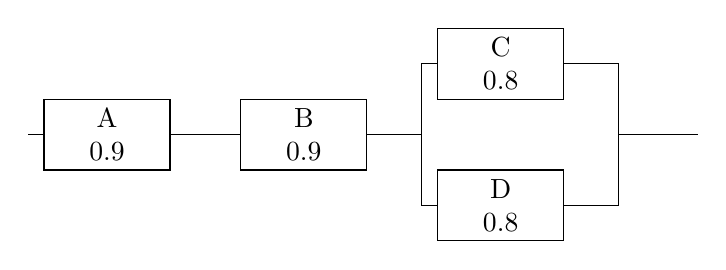
\begin{tikzpicture}[
    scale=1,
    every node/.style={
        draw,
        rectangle,
        minimum width=1.6cm,
        minimum height=0.9cm,
        align=center
    }
]

% Nodes
\node (A) at (0,0) {A \\ 0.9};
\node (B) at (2.5,0) {B \\ 0.9};

\node (C) at (5,0.9) {C \\ 0.8};
\node (D) at (5,-0.9) {D \\ 0.8};

% Connections
\draw (-1,0) -- (A);
\draw (A) -- (B);
\draw (B) -- (4,0);

\draw (4,0) -- (4,0.9) -- (C);
\draw (4,0) -- (4,-0.9) -- (D);

\draw (C) -- (6.5,0.9) -- (6.5,0);
\draw (D) -- (6.5,-0.9) -- (6.5,0);

\draw (6.5,0) -- (7.5,0);

\end{tikzpicture}
\end{center}

\[
P(A)=0.9,\quad P(B)=0.9,\quad P(C)=0.8,\quad P(D)=0.8
\]
\subsubsection*{(a) Probability the entire system works}

The system works if $A$ and $B$ work and either $C$ or $D$ works.

\[
\begin{aligned}
P(\text{system works})
&= P(\text{all work}) 
+ P(A,B,C \text{ work}, D \text{ does not}) \\
&\quad + P(A,B,D \text{ work}, C \text{ does not})
\end{aligned}
\]

\[
= (0.9)(0.9)(0.8)(0.8)
+ (0.9)(0.9)(0.8)(1-0.8)
+ (0.9)(0.9)(0.8)(1-0.8)
\]

\[
\boxed{
P(\text{system works}) = 0.7776
}
\]

\subsubsection*{(b) Conditional probability}

\[
P(C^c \mid \text{system works})
= \frac{P(C^c \cap \text{system works})}{P(\text{system works})}
\]

\[
P(C^c \cap \text{system works})
= (0.9)(0.9)(0.8)(1-0.8)
\]

\[
\boxed{
P(C^c \mid \text{system works})
= \frac{(0.9)(0.9)(0.8)(1-0.8)}{0.7776}
= 0.16
}
\]

\begin{center}
\begin{tcolorbox}[
    colback=softpink!5,
    colframe=softpink!70!black,
    coltitle=black,
    colbacktitle=softpink,
    title=\textbf{Theorem of Total Probability},
    boxrule=0.8pt,
    arc=6pt,
    width=0.9\textwidth
]

Let $B_1, B_2, \ldots, B_k$ be a \underline{partition} of the sample space $S$ such that
$P(B_i) > 0$ for all $i$.
Then for any event $A \subseteq S$,

\[
\boxed{
P(A)
= \sum_{i=1}^{k} P(A \mid B_i)\,P(B_i)
= \sum_{i=1}^{k} P(A \cap B_i)
}
\]

\end{tcolorbox}
\end{center}

\begin{center}
\begin{tcolorbox}[
    colback=softpink!5,
    colframe=softpink!70!black,
    coltitle=black,
    colbacktitle=softpink,
    title=\textbf{Theorem: Bayes' Rule (1701--1761)},
    boxrule=0.8pt,
    arc=6pt,
    width=0.9\textwidth
]

Let $B_1, B_2, \ldots, B_k$ be a \underline{partition} of the sample space $S$ such that
$P(B_i) > 0$ for $i = 1,\ldots,k$.
For any event $A \subseteq S$ with $P(A) > 0$,

\[
\boxed{
P(B_r \mid A)
= \frac{P(B_r \cap A)}{\sum_{i=1}^{k} P(B_i \cap A)}
= \frac{P(B_r)\,P(A \mid B_r)}{\sum_{i=1}^{k} P(B_i)\,P(A \mid B_i)},
\quad r = 1,\ldots,k
}
\]

\end{tcolorbox}
\end{center}

\begin{figure}[H]
\centering
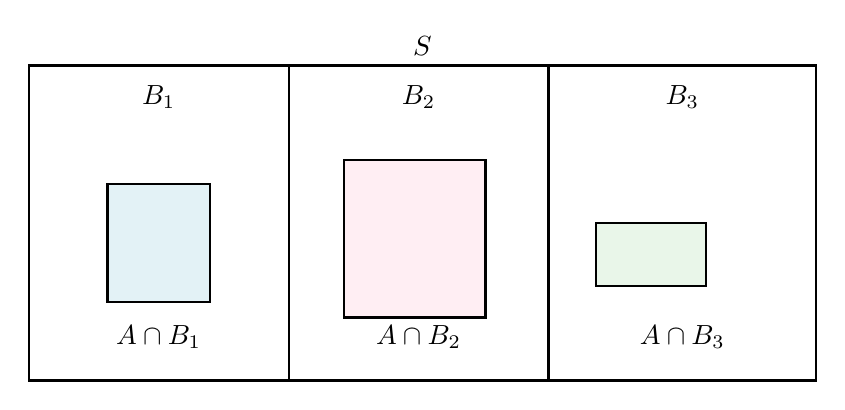
\begin{tikzpicture}[scale=1]

% Sample space
\draw[thick] (0,0) rectangle (10,4);
\node[above] at (5,4) {$S$};

% Partition blocks (B1, B2, B3)
\draw[thick] (0,0) rectangle (3.3,4);
\draw[thick] (3.3,0) rectangle (6.6,4);
\draw[thick] (6.6,0) rectangle (10,4);

\node at (1.65,3.6) {$B_1$};
\node at (4.95,3.6) {$B_2$};
\node at (8.3,3.6) {$B_3$};

% A cap Bi regions (filled baby candy colors)
\fill[babyblue!40,   opacity=0.85] (1.0,1.0) rectangle (2.3,2.5);
\fill[babypink!40,   opacity=0.85] (4.0,0.8) rectangle (5.8,2.8);
\fill[babygreen!40,  opacity=0.85] (7.2,1.2) rectangle (8.6,2.0);

% Optional: outline the A cap Bi regions for clarity
\draw[thick] (1.0,1.0) rectangle (2.3,2.5);
\draw[thick] (4.0,0.8) rectangle (5.8,2.8);
\draw[thick] (7.2,1.2) rectangle (8.6,2.0);

% Labels for intersections
\node at (1.65,0.55) {$A \cap B_1$};
\node at (4.95,0.55) {$A \cap B_2$};
\node at (8.3,0.55) {$A \cap B_3$};

\end{tikzpicture}
\caption{Partition of $S$ into $B_1,B_2,B_3$ with shaded regions $A\cap B_i$}
\end{figure}

\subsection*{Example (Medical Test)}

The fraction of people in a population who have a certain disease is $0.01$.

\[
P(D) = 0.01, \quad P(D^c) = 0.99
\]

The test characteristics are:
\[
P(\text{test says } D \mid D^c) = 0.05
\quad \text{(false positive rate)}
\]

\[
P(\text{test says } D^c \mid D) = 0.20
\quad \text{(false negative rate)}
\]

Thus,
\[
P(\text{test says } D \mid D) = 1 - 0.20 = 0.80
\]

\textit{
\underline{Note:}
$1 - P(\text{test says } D^c \mid D)$ is called the \underline{sensitivity} of the test,
and $1 - P(\text{test says } D \mid D^c)$ is called the \underline{specificity}.
}
\begin{center}
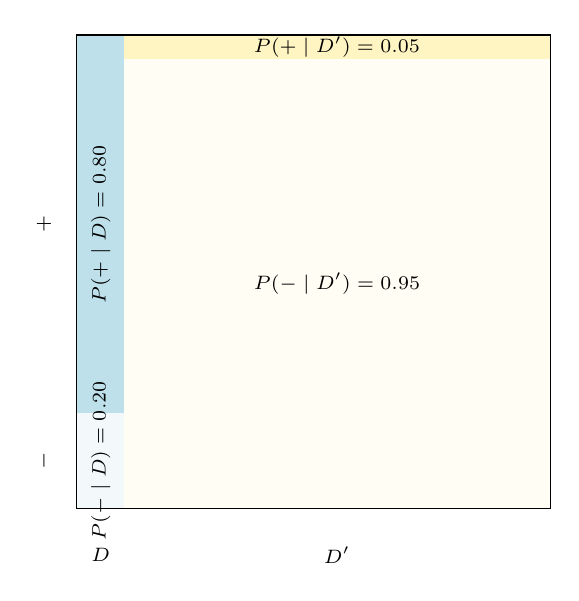
\begin{tikzpicture}[scale=6]

% Outer square (whole population)
\draw[thick] (0,0) rectangle (1,1);

% Vertical split: D vs D'
\draw[thick] (0.1,0) -- (0.1,1);

% Horizontal splits (test result splits within each group)
\draw[thick] (0,0.20) -- (0.1,0.20);      % within D
\draw[thick] (0.1,0.95) -- (1,0.95);      % within D'

% Fill regions
\fill[babyblue!80]   (0,0.20) rectangle (0.1,1);      % D and +
\fill[babyblue!15]   (0,0) rectangle (0.1,0.20);      % D and -

\fill[babyyellow!80]  (0.1,0.95) rectangle (1,1);      % D' and +
\fill[babyyellow!15]  (0.1,0) rectangle (1,0.95);      % D' and -

% Labels inside rectangles
\node[rotate=90] at (0.05,0.60) {\scriptsize $P(+\mid D)=0.80$};
\node[rotate=90] at (0.05,0.10) {\scriptsize $P(-\mid D)=0.20$};

\node at (0.55,0.975) {\scriptsize $P(+\mid D')=0.05$};
\node at (0.55,0.475) {\scriptsize $P(-\mid D')=0.95$};

% Bottom labels
\node at (0.05,-0.1) {\scriptsize $D$};
\node at (0.55,-0.1) {\scriptsize $D'$};

% Side labels
\node[rotate=90] at (-0.07,0.60) {\scriptsize $+$};
\node[rotate=90] at (-0.07,0.10) {\scriptsize $-$};

\end{tikzpicture}
\end{center}



\subsubsection*{(a) Probability the test says disease}

\[
P(\text{test says } D)
= P(D \cap \text{test says } D)
+ P(D^c \cap \text{test says } D)
\]

\[
= P(\text{test says } D \mid D)P(D)
+ P(\text{test says } D \mid D^c)P(D^c)
\]

\[
= (0.80)(0.01) + (0.05)(0.99)
= 0.0575
\]


\subsubsection*{(b) Probability of disease given positive test}

\[
P(D \mid \text{test says } D)
= \frac{P(D \cap \text{test says } D)}{P(\text{test says } D)}
\]

\[
= \frac{P(\text{test says } D \mid D)P(D)}{0.0575}
= \frac{(0.80)(0.01)}{0.0575}
\]

\[
\boxed{
P(D \mid \text{test says } D) \approx 0.139
}
\]


\subsubsection*{(c) Probability of disease given negative test}

\[
P(D \mid \text{test says } D^c)
= \frac{P(D \cap \text{test says } D^c)}{P(\text{test says } D^c)}
\]

\[
= \frac{P(\text{test says } D^c \mid D)P(D)}{1 - P(\text{test says } D)}
\]

\[
= \frac{(0.20)(0.01)}{1 - 0.0575}
\]

\[
\boxed{
P(D \mid \text{test says } D^c) \approx 0.00212
}
\]

\section*{Chapter 3 — January 19}
\label{chap:three}
\section*{Random Variables and Their Interpretation}
\label{sec:rv_definition}

\textbf{Definition:}  
A \underline{random variable (r.v.)} is a rule that assigns a \textbf{real number} to each outcome in the sample space.
\\
\textbf{Alternative definition:}  A \underline{random variable} is a function that takes the outcome of an experiment and assigns it a number so that probabilities can be calculated.

\vspace{0.5em}

\subsection*{Example 1: Three Electronic Components}

Each component is classified as either defective (D) or non-defective (N).

\[
S = \{NNN, DNN, NDN, NND, DDN, DND, NDD, DDD\}
\]

\begin{itemize}
\item \textbf{Defective (D):} the component does not meet required specifications and fails inspection.
\item \textbf{Non-defective (N):} the component meets specifications and passes inspection.
\end{itemize}

Define the random variable
\[X= \text{number of defective components}.
\]

Then:
\[
\begin{aligned}
X = 0 &\quad \text{for } \{NNN\} \\
X = 1 &\quad \text{for } \{DNN, NDN, NND\} \\
X = 2 &\quad \text{for } \{DDN, DND, NDD\} \\
X = 3 &\quad \text{for } \{DDD\}
\end{aligned}
\]

Thus, the possible values of \(X\) are:
\[
\{0,1,2,3\}.
\]

\vspace{0.5em}

\subsection*{Example 2: One Component (Dummy Variable)}

\[
S = \{D, N\}
\]

Define the random variable
\[
X =
\begin{cases}
1, & \text{if the component is defective (D)} \\
0, & \text{if the component is non-defective (N)}
\end{cases}
\]

This is called a \textbf{dummy variable} because the outcome is categorical, but is encoded numerically. 
\\A \underline{dummy variable} is a special type of random variable that assigns numerical labels to categorical outcomes, where the numbers have no quantitative meaning beyond identification.


\vspace{0.5em}

\subsection*{Discrete Random Variables}
\label{sec:rv_types}


\textbf{Definition:}  
A random variable is called \underline{discrete} if its set of possible values is \textbf{countable} (finite or countably infinite).

\vspace{0.5em}

\vspace{0.5em}\subsection*{Example 3: Sampling Until First Defective}

Components are tested one(independently) at a time until the first defective component is observed.

\[
S = \{D,\ ND,\ NND,\ NNND,\ldots\}
\]

Define
\[X = \text{number of components tested until the first defective}.
\]

Then:
\[
\begin{aligned}
X = 1 &\quad \text{for } \{D\} \\
X = 2 &\quad \text{for } \{ND\} \\
X = 3 &\quad \text{for } \{NND\} \\
&\vdots
\end{aligned}
\]

Hence,
\[
X = 1,2,3,\ldots
\]

Since the possible values can be listed, \(X\) is a \underline{discrete random variable}.

\textbf{Non-discrete version of the same experiment:}

Define
\[
Y = \text{time (in seconds) until the first defective component is observed}.
\]

Since \(Y\) can take any real value in \([0,\infty)\), it cannot be listed and is therefore a \underline{continuous (non-discrete) random variable}.


\subsection*{Discrete vs.\ Continuous Random Variables}

\begin{center}
\begin{tabular}{|c|c|}
\hline
\textbf{Discrete Random Variable} & \textbf{Continuous Random Variable} \\
\hline
Counts things & Measures things \\
\hline
Possible values are countable & Possible values fill an interval \\
\hline
$P(X = x)$ can be $> 0$ & $P(X = x) = 0$ for all $x$ \\
\hline
Uses a probability mass function (PMF) & Uses a probability density function (PDF) \\
\hline
\end{tabular}
\end{center}

\subsection*{Probability Mass Function (PMF)}
\label{sec:pmf}


\textbf{Definition:}  

Let \(X\) be a discrete random variable.  
The \underline{probability mass function (PMF)} of \(X\), denoted \(f(x)\), is defined by:

\[
\boxed{
\begin{aligned}
&1)\quad f(x) \ge 0 \quad \text{for all } x \\
&2)\quad \sum_x f(x) = 1
\end{aligned}
}
\]


\textbf{Note:}
\begin{itemize}
\item Capital \(X\): random variable
\item Lowercase \(x\): a specific value
\end{itemize}

\subsection*{Bernoulli and Binomial Random Variables}
\vspace{0.5em}

\subsubsection*{I. Bernoulli Random Variable (Single Trial)}

A \underline{Bernoulli random variable: X} models a single experiment with only two possible outcomes: success or failure.

\[
X =
\begin{cases}
1, & \text{success} \\
0, & \text{failure}
\end{cases}
\]

If \(p = P(X=1)\), then the PMF is
\[
\begin{array}{c|cc}
x & 0 & 1 \\
\hline
P(X=x) & 1-p & p
\end{array}
\]

Here, \(p\) is the probability of success (e.g.\ observing a defective component).

\vspace{1em}

\subsubsection*{Binomial Random Variable (Multiple Bernoulli Trials)}

The \underline{binomial random variable} extends the Bernoulli case to multiple independent trials.

\textbf{Definition:}  

A random variable \(X\) is called a binomial random variable if it represents the number of successes in \(n\) independent Bernoulli trials, each with success probability \(p\).

\[
X = \text{number of successes in } n \text{ trials}
\]

In this case,
\[
X \sim \text{Bin}(n,p)
\]
and the probability mass function is
\[
\fbox{
$P(X = x) = \binom{n}{x} p^x (1-p)^{n-x}, \quad x = 0,1,\ldots,n.$
}
\]

\vspace{0.5em}

\subsubsection*{Conditions for a Binomial Model}

A binomial model applies only if:
\begin{itemize}
\item each trial has exactly two outcomes (success or failure),
\item the probability of success \(p\) is the same for every trial,
\item the trials are independent,
\item the number of trials \(n\) is fixed.
\end{itemize}

\vspace{1em}

\subsubsection*{Example: Three Components Tested}

Assume each component is defective with probability
\[
p = 0.1, \quad n = 3.
\]
where p = P(a single component is defective), n = number of trials 

Let
\[
X = \text{number of defective components}.
\]

\[
\begin{array}{c|c}
x & P(X = x) \\ \hline
0 & \binom{3}{0}(0.9)^3 = 0.729 \\
1 & \binom{3}{1}(0.1)(0.9)^2 = 0.243 \\
2 & \binom{3}{2}(0.1)^2(0.9) = 0.027 \\
3 & \binom{3}{3}(0.1)^3 = 0.001
\end{array}
\]

\[
0.729 + 0.243 + 0.027 + 0.001 = 1.
\]


\begin{center}
\cue[
    xlabel={$x$},
    ylabel={$P(X=x)$},
    title={\textbf{PMF of $X$}},
    ymin=0,
    ymax=0.8,
    xtick={0,1,2,3},
    enlarge x limits=0.2
]{
    \addplot[ybar, fill=babyblue,   draw=black] coordinates {(0,0.729)};
    \addplot[ybar, fill=babypink,   draw=black] coordinates {(1,0.243)};
    \addplot[ybar, fill=babyyellow, draw=black] coordinates {(2,0.027)};
    \addplot[ybar, fill=babyorange, draw=black] coordinates {(3,0.001)};

    % Value labels
    \node at (axis cs:0,0.729) [above] {$0.729$};
    \node at (axis cs:1,0.243) [above] {$0.243$};
    \node at (axis cs:2,0.027) [above] {$0.027$};
    \node at (axis cs:3,0.001) [above] {$0.001$};
}
\end{center}

\subsection*{Geometric Random Variable}

\subsubsection*{Example: Sampling Until First Defective}

Components are sampled one at a time until the first defective component is observed.  
Assume the probability that a component is defective is
\[
p = 0.1.
\]

Define the random variable
\[
X = \text{number of samples collected until the first defective}.
\]

\[
\begin{array}{c|c}
x & P(X = x) = f(x) \\ \hline
1 & 0.1 \\
2 & 0.9(0.1) \\
3 & 0.9^2(0.1) \\
\vdots & \vdots
\end{array}
\]

\subsubsection*{Geometric Random Variable}

\textbf{Definition:}  

A random variable \(X\) is called a \underline{geometric random variable} if it represents the number of trials needed to obtain the first success in a sequence of independent Bernoulli trials with success probability \(p\).

\[
\boxed{
P(X = x) = (1-p)^{x-1}p, \quad x = 1,2,3,\ldots
}
\]

In this example,
\[
P(X = x) = 0.9^{x-1}(0.1).
\]

\subsubsection*{Verification That Probabilities Sum to 1}

\[
\sum_{x=1}^{\infty} 0.9^{x-1}(0.1)
= 0.1 \sum_{x=0}^{\infty} 0.9^{x}
= 0.1 \left( \frac{1}{1-0.9} \right)
= 1.
\]

\subsection*{Cumulative Distribution Function (CDF)}
\label{sec:cdf}
\label{sec:cdf_discrete}


\textbf{Definition:}  

The \underline{cumulative distribution function (CDF)} of a discrete random variable \(X\) with PMF \(f(x)\) is defined as
\[
\boxed{
F(x) = P(X \le x) = \sum_{t \le x} f(t), \quad -\infty < x < \infty.
}
\]


\subsection*{Example: Binomial Distribution (Three Components)}

Let \(X\) be the number of defective components when three components are tested, with
\[
P(X=0)=0.729,\quad P(X=1)=0.243,\quad P(X=2)=0.027,\quad P(X=3)=0.001.
\]

\[
\begin{aligned}
F(0) &= P(X \le 0) = 0.729 \\
F(1) &= P(X \le 1) = 0.729 + 0.243 = 0.972 \\
F(2) &= P(X \le 2) = 0.729 + 0.243 + 0.027 = 0.999 \\
F(3) &= P(X \le 3) = 0.729 + 0.243 + 0.027 + 0.001 = 1
\end{aligned}
\]

Thus, the CDF can be written as
\[
F(x) =
\begin{cases}
0, & x < 0 \\
0.729, & 0 \le x < 1 \\
0.972, & 1 \le x < 2 \\
0.999, & 2 \le x < 3 \\
1, & x \ge 3
\end{cases}
\]

\subsection*{Properties of the CDF}

\begin{itemize}
\item \(F(x)\) is \underline{monotone non-decreasing}.
\item If \(x < y\), then \(F(x) \le F(y)\).
\item \(0 \le F(x) \le 1\).
\end{itemize}
\textbf{Note:} A function is \textbf{monotone} non-decreasing if its value never decreases as the input increases.


\subsection*{Using the CDF to Compute Probabilities}

For \(a < b\),
\[
P(a < X \le b) = F(b) - F(a).
\]

Example:
\[
P(0 < X \le 2) = F(2) - F(0) = 0.999 - 0.729 = 0.27.
\]
\subsection*{CDF Histogram (Step Function)}

\begin{center}
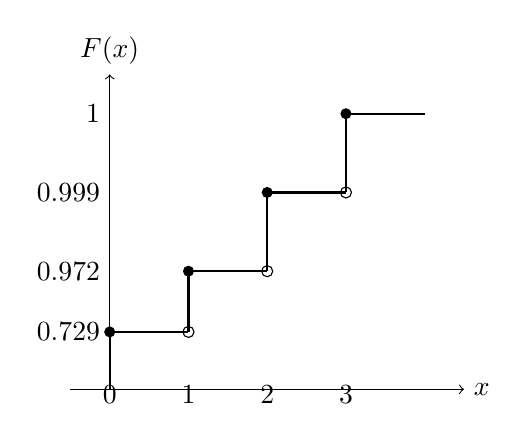
\begin{tikzpicture}

% Axes
\draw[->] (-0.5,0) -- (4.5,0) node[right] {$x$};
\draw[->] (0,0) -- (0,4) node[above] {$F(x)$};

% Horizontal steps
\draw[thick] (0,0.729) -- (1,0.729);
\draw[thick] (1,1.5) -- (2,1.5);
\draw[thick] (2,2.5) -- (3,2.5);
\draw[thick] (3,3.5) -- (4,3.5);

% Vertical jumps
% Vertical jumps (correct)
\draw[thick] (0,0) -- (0,0.729);
\draw[thick] (1,0.729) -- (1,1.5);
\draw[thick] (2,1.5) -- (2,2.5);
\draw[thick] (3,2.5) -- (3,3.5);

% Dots (right-continuous)
\fill (0,0.729) circle (2pt);
\fill (1,1.5) circle (2pt);
\fill (2, 2.5) circle (2pt);
\fill (3,3.5) circle (2pt);

% Open dots (left limits)
\draw (1,0.729) circle (2pt);
\draw (2,1.5) circle (2pt);
\draw (3,2.5) circle (2pt);

% Labels
\node[left] at (0,0.729) {$0.729$};
\node[left] at (0,1.5) {$0.972$};
\node[left] at (0,2.5) {$0.999$};
\node[left] at (0,3.5) {$1$};

\node at (0,-0.07) {0};
\node at (1,-0.07) {1};
\node at (2,-0.07) {2};
\node at (3,-0.07) {3};

\end{tikzpicture}
\end{center}

\textbf{Note:} For a discrete random variable, the \underline{PMF} is drawn as a bar chart since it shows probabilities at individual points, while the \underline{CDF} is drawn as a step function since it represents cumulative probability and is monotone non-decreasing.


\section*{Chapter 3 — January 21}
\subsection*{Review}

\begin{enumerate}
    \item \underline{\textit{Random Variable (RV), $X$}}:  
    A random variable assigns a real number to each outcome.

    \item \underline{\textit{Discrete Random Variable}}:  
    If $X$ is discrete,
    \begin{itemize}
        \item $P(X = x) = f(x)$
        \item $f(x)$ is the \underline{\textit{probability mass function (PMF)}}
        \item $f(x) \ge 0$
        \item $\displaystyle \sum_x f(x) = 1$
    \end{itemize}

    \item \underline{\textit{Cumulative Distribution Function (CDF), $F(x)$}}:  
    \begin{itemize}
        \item $F(x) = P(X \le x)$
        \item If $X$ is discrete:
        \[
        F(x) = \sum_{t \le x} f(t), \quad -\infty < x < \infty
        \]
    \end{itemize}
\end{enumerate}

\subsection*{Continuous Sample Space and Continuous Random Variables}
\label{sec:continuous_rv}


If the sample space contains an infinite number of outcomes equal to the number of points on a line segment, it is called a \underline{continuous sample space}.

A \underline{continuous random variable} has
\[
\boxed{
P(X = x) = 0 \quad \text{for all } x,
}
\]
so probabilities are computed over intervals instead of single values.
\\

\textbf{*Alternative definition}: A \underline{continuous sample} space contains infinitely many outcomes, like the points on a line segment.  
For a \underline{continuous random variable}, the probability of taking any exact value is zero, i.e.\ $P(X=x)=0$ for all $x$.  
Therefore, probabilities are computed over intervals rather than at single points.


\subsection*{Probability Density Function (PDF)}


A function \(f(x)\) is called a \underline{probability density function (PDF)} of a continuous random variable \(X\), defined over \(\mathbb{R}\), if:

\begin{center}
\fbox{
\begin{minipage}{0.9\linewidth}
\begin{enumerate}
    \item \(f(x) \ge 0\) for all \(x \in \mathbb{R}\)
    \item \(\displaystyle \int_{-\infty}^{\infty} f(x)\,dx = 1\)
    \item For any \(a < b\),
    \[
    P(a < X < b) = \int_a^b f(x)\,dx
    \]
\end{enumerate}
\end{minipage}
}
\end{center}

For continuous random variables,
\[
P(a < X < b)
= P(a \le X \le b)
= P(a \le X < b)
= P(a < X \le b).
\]


\[
\boxed{P(X = a) = 0}
\]

because a single point has zero area under the probability density function.

% In your preamble:
% \usepackage{tikz}
% \usetikzlibrary{patterns}

\begin{center}
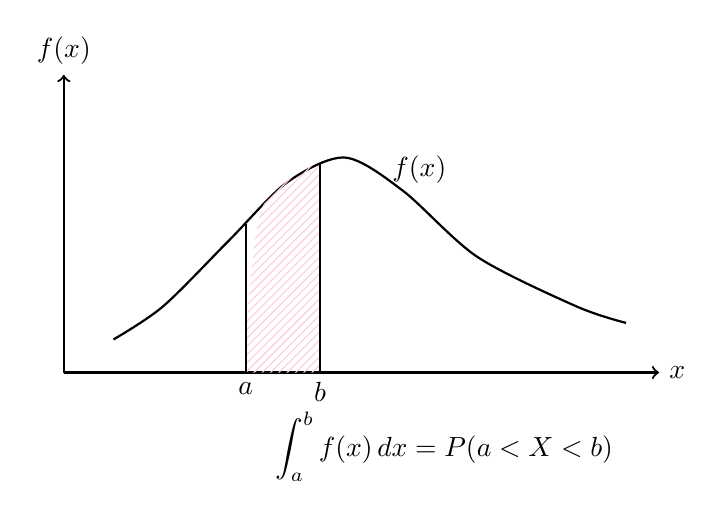
\begin{tikzpicture}[scale=1.05]

% Axes
\draw[->, thick] (0,0) -- (7.2,0) node[right] {$x$};
\draw[->, thick] (0,0) -- (0,3.6) node[above] {$f(x)$};

% Parameters for a and b (choose any values between 0 and 7)
\def\xa{2.2}
\def\xb{3.1}

% A smooth "pdf-like" curve (hand-drawn look, not an exact function)
\draw[thick]
plot[smooth] coordinates {
(0.6,0.4) (1.2,0.8) (2.0,1.6) (2.7,2.3)
(3.4,2.6) (4.1,2.2) (5.0,1.4) (6.2,0.8) (6.8,0.6)
};

% Label on the curve
\node at (4.3,2.45) {$f(x)$};

% Shaded region between a and b under the curve
\fill[pattern=north east lines, pattern color=babypink]
(\xa,0)
--
plot[smooth] coordinates {
(\xa, {0.4 + 0.0})
(2.4,2.0)
(\xb,2.55)
}
--
(\xb,0)
-- cycle;

% Vertical lines at a and b
\draw[thick] (\xa,0) -- (\xa,1.8);
\draw[thick] (\xb,0) -- (\xb,2.52);

% Labels a and b on x-axis
\node[below] at (\xa,0) {$a$};
\node[below] at (\xb,0) {$b$};

% Integral annotation
\node[align=left] at (4.6,-0.9)
{$\displaystyle \int_{a}^{b} f(x)\,dx = P(a<X<b)$};

\end{tikzpicture}
\end{center}

\subsection*{Example: Uniform Distribution}

Let the probability density function be
\[
f(x) =
\begin{cases}
c, & 5 < x < 10, \\
0, & \text{otherwise}.
\end{cases}
\]

\textbf{1) Determine the value of \(c\)}

Since \(f(x)\) is a \underline{probability density function}, the total area under the curve must equal 1:
\[
\int_{-\infty}^{\infty} f(x)\,dx = 1.
\]

Because \(f(x)=0\) outside the interval \((5,10)\),
\[
\int_5^{10} c\,dx = 1.
\]

Evaluating the integral,
\[
c(10-5) = 1 \quad \Rightarrow \quad c = \frac{1}{5}.
\]

Thus,
\[
f(x) =
\begin{cases}
\frac{1}{5}, & 5 < x < 10, \\
0, & \text{otherwise}.
\end{cases}
\]

\begin{center}
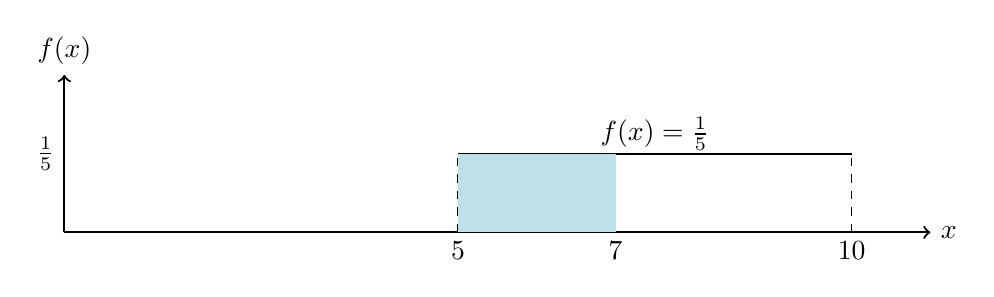
\begin{tikzpicture}[scale=1.0]
\draw[->, thick] (0,0) -- (11,0) node[right] {$x$};
\draw[->, thick] (0,0) -- (0,2) node[above] {$f(x)$};

% rectangle for uniform pdf
\draw[thick] (5,1) -- (10,1);
\draw[dashed] (5,0) -- (5,1);
\draw[dashed] (10,0) -- (10,1);

% shading for P(X<7)
\fill[babyblue!80] (5,0) rectangle (7,1);

% labels
\node[left] at (0,1) {$\frac{1}{5}$};
\node[below] at (5,0) {$5$};
\node[below] at (7,0) {$7$};
\node[below] at (10,0) {$10$};

\node at (7.5,1.25) {$f(x)=\frac{1}{5}$};
\end{tikzpicture}
\end{center}

\textbf{2): Compute \(P(X<7)\)}

\textbf{Formula used:}
\[
P(a<X<b) = \int_a^b f(x)\,dx.
\]

Applying this formula,
\[
P(X<7)
= \int_5^7 \frac{1}{5}\,dx
= \frac{1}{5}(7-5)
= \frac{2}{5}.
\]

\subsection*{CDF for Continuous Random Variables}
\label{sec:cdf_continuous}

\textbf{Def:} Let \(X\) be a \underline{continuous random variable} with \underline{pdf: probability density function} \(f(x)\).  
The \underline{cumulative distribution function (CDF)} is
\[
F(x) = P(X \le x) = \int_{-\infty}^{x} f(t)\,dt.
\]

\textbf{Consequently:}
\begin{center}
\fbox{
\begin{minipage}{0.9\linewidth}
\[
f(x) = \frac{d}{dx}F(x),
\qquad
P(a < X < b) = F(b) - F(a).
\]
\end{minipage}
}
\end{center}

\subsection*{Example}

Let \(X\) be the time until a chemical reaction is complete (in msec). Suppose the CDF is
\[
F(x)=
\begin{cases}
0, & x<0,\\
1-e^{-0.01x}, & x \ge 0.
\end{cases}
\]

\textbf{(a) Find the pdf.}

Use \(\,f(x)=\dfrac{d}{dx}F(x)\).

For \(x<0\), \(F(x)=0\), so
\[
f(x)=0.
\]

For \(x \ge 0\),
\[
f(x)=\frac{d}{dx}\left(1-e^{-0.01x}\right)
= 0.01e^{-0.01x}.
\]

Therefore,
\[
f(x)=
\begin{cases}
0, & x<0,\\
0.01e^{-0.01x}, & x \ge 0.
\end{cases}
\]

\textbf{(b) Find \(P(X<200)\).}

Use the CDF directly:
\[
P(X<200)=F(200)=1-e^{-0.01(200)}=1-e^{-2}\approx 0.8647.
\]

\textbf{(c) Check if this is a valid CDF.}
\begin{center}
\begin{tcolorbox}[
    colback=softpink!3,
    colframe=softpink!70!black,
    coltitle=black,
    colbacktitle=softpink,
    title=\textbf{Theorem: Properties of a Cumulative Distribution Function},
    width=0.9\textwidth
]
A function \(F(x)\) is a \underline{valid cumulative distribution function (CDF)} if and only if:
\begin{itemize}
    \item \(0 \le F(x) \le 1\) for all \(x\)
    \item \(F(x)\) is \underline{monotone non-decreasing}, i.e.
    \[
    x \le y \implies F(x) \le F(y)
    \]
    \item \(\displaystyle \lim_{x \to -\infty} F(x) = 0\)
    \item \(\displaystyle \lim_{x \to \infty} F(x) = 1\)
\end{itemize}
\end{tcolorbox}
\end{center}

For this \(F(x)\):
\[
\lim_{x\to -\infty}F(x)=0,
\qquad
\lim_{x\to \infty}F(x)=1,
\]
and for \(x\ge 0\), \(1-e^{-0.01x}\) increases as \(x\) increases, so \(F(x)\) is monotone non-decreasing.

Thus, \(F(x)\) is a valid CDF.
\subsection*{Joint Probability Distributions (Discrete)}
\label{sec:joint}
\label{sec:joint_discrete}


\textbf{Def:}  
The function \(f(x,y)\) is a \underline{joint probability mass function (PMF)} of discrete random variables \(X\) and \(Y\) if:

\begin{center}
\fbox{
\begin{minipage}{0.9\linewidth}
\begin{enumerate}
    \item \(f(x,y) \ge 0\) for all \((x,y)\)
    \item \(\displaystyle \sum_x \sum_y f(x,y) = 1\)
    \item \(P(X=x, Y=y) = f(x,y)\)
\end{enumerate}
\end{minipage}
}
\end{center}

That is, \(f(x,y)\) gives the probability that the two random variables \(X\) and \(Y\) take the values \(x\) and \(y\) \emph{simultaneously}.

For any region \(A\) in the \(xy\)-plane,
\[
\boxed{
P\big((X,Y) \in A\big) = \sum_{(x,y)\in A} f(x,y)
}
\]


\subsection*{Example: Pen Refills}

Two refills are selected at random and without replacement from a box containing:
\begin{itemize}
    \item 3 blue refills
    \item 2 red refills
    \item 3 green refills
\end{itemize}

Define the random variables
\[
X = \text{number of blue refills selected},
\qquad
Y = \text{number of red refills selected}.
\]

The total number of possible selections is
\[
\binom{8}{2}.
\]

\subsection*{Joint PMF Table}

For each pair \((x,y)\),
\[
f(x,y) = \frac{\text{number of favorable outcomes}}{\binom{8}{2}}.
\]

\begin{center}
\renewcommand{\arraystretch}{2.2}
\begin{tabular}{c|ccc|c}
\(X \backslash Y\) & 0 & 1 & 2 & Row Total \\ \hline
0 &
$\dfrac{\binom{3}{2}}{\binom{8}{2}}$ &
$\dfrac{\binom{2}{1}\binom{3}{1}}{\binom{8}{2}}$ &
$\dfrac{\binom{2}{2}}{\binom{8}{2}}$ &
$\dfrac{\binom{5}{2}}{\binom{8}{2}}$
\\
1 &
$\dfrac{\binom{3}{1}\binom{3}{1}}{\binom{8}{2}}$ &
$\dfrac{\binom{3}{1}\binom{2}{1}}{\binom{8}{2}}$ &
$0$ &
$\dfrac{15}{\binom{8}{2}}$
\\
2 &
$\dfrac{\binom{3}{2}}{\binom{8}{2}}$ &
$0$ &
$0$ &
$\dfrac{3}{\binom{8}{2}}$
\\ \hline
Column Total &
$\dfrac{15}{\binom{8}{2}}$ &
$\dfrac{12}{\binom{8}{2}}$ &
$\dfrac{1}{\binom{8}{2}}$ &
$1$
\end{tabular}
\end{center}

\subsection*{Marginal Distributions}
\label{sec:marginal}

\textbf{Def:}  
Let \(f(x,y)\) be the joint PMF of \(X\) and \(Y\).

The \underline{marginal PMF of \(X\)} is obtained by summing over all values of \(Y\):
\[
g(x) = \sum_y f(x,y).
\]

The \underline{marginal PMF of \(Y\)} is obtained by summing over all values of \(X\):
\[
h(y) = \sum_x f(x,y).
\]

\textbf{Marginal example:}
\[
P(X=1) = \sum_y P(X=1, Y=y).
\]


\subsection*{Conditional Distributions (Discrete)}
\label{sec:conditional}

\textbf{Def:}  
The \underline{conditional PMF of \(Y\) given \(X=x\)} is
\[
f_{Y|X}(y|x) = \frac{f(x,y)}{g(x)}, \quad g(x) > 0.
\]

Similarly, the \underline{conditional PMF of \(X\) given \(Y=y\)} is
\[
f_{X|Y}(x|y) = \frac{f(x,y)}{h(y)}, \quad h(y) > 0.
\]


\subsection*{Example: Conditional Probabilities}

\begin{enumerate}
    \item 
    \[
    P(Y=1 \mid X=1)
    = \frac{P(X=1,Y=1)}{P(X=1)}
    = \frac{3/28}{15/28}
    = \frac{3}{15}.
    \]

    \item
    \[
    P(X=0 \mid Y=1)
    = \frac{P(X=0,Y=1)}{P(Y=1)}
    = \frac{9/28}{15/28}
    = \frac{9}{15}.
    \]

    \item
    \[
    P(Y=2 \mid X=1) = 0.
    \]
\end{enumerate}

Check:
\[
\sum_y P(Y=y \mid X=1) = 1.
\]


\subsection*{Review: Chapter 3 — Random Variables}

\begin{enumerate}
\item \textit{\underline{Random Variable}}  
A random variable is a function that maps outcomes of an experiment to real numbers.
    \begin{itemize}
        \item Domain: sample space outcomes
        \item Range: real numbers
        \item Can be \textbf{discrete} or \textbf{continuous}
    \end{itemize}

\item \textit{\underline{Probability Mass Function (PMF)}}  
\label{sec:pmf}
\label{sec:pmf_discrete}
The PMF of a discrete random variable \(X\) is
\[
f_X(x) = P(X = x)
\]
    \begin{itemize}
        \item Only for discrete random variables
        \item \(f_X(x) \ge 0\)
        \item \(\sum_x f_X(x) = 1\)
    \end{itemize}

\item \textit{\underline{Probability Density Function (PDF)}}  
\label{sec:pdf}
For a continuous random variable \(X\), probability is defined by
\[
P(a \le X \le b) = \int_a^b f_X(x)\,dx
\]
    \begin{itemize}
        \item Only for continuous random variables
        \item Area under the curve gives probability
        \item \(P(X = x) = 0\)
    \end{itemize}

\item \textit{\underline{Cumulative Distribution Function (CDF)}}  
The CDF is defined as
\[
F_X(x) = P(X \le x)
\]
    \begin{itemize}
        \item Discrete: \(F(x)=\sum_{t \le x} f(t)\)
        \item Continuous: \(F(x)=\int_{-\infty}^{x} f(t)\,dt\)
        \item \(0 \le F(x) \le 1\), non-decreasing
    \end{itemize}

\item \textit{\underline{Joint Distribution}}  
\label{sec:joint_continuous}
The joint distribution describes probabilities involving two random variables \(X\) and \(Y\).
    \begin{itemize}
        \item Discrete: \(f_{X,Y}(x,y)=P(X=x,Y=y)\)
        \item Continuous: joint PDF \(f_{X,Y}(x,y)\)
    \end{itemize}

\item \textit{\underline{Marginal Distribution}}  
A marginal distribution is obtained by eliminating the other variable.
    \begin{itemize}
        \item \(f_X(x)=\sum_y f_{X,Y}(x,y)\) or \(f_X(x)=\int f_{X,Y}(x,y)\,dy\)
        \item \(f_Y(y)=\sum_x f_{X,Y}(x,y)\) or \(f_Y(y)=\int f_{X,Y}(x,y)\,dx\)
    \end{itemize}
\end{enumerate}

\subsection*{Joint Probability Density Function (Continuous)}

\textbf{Def:}  
A function \(f(x,y)\) is a \underline{joint probability density function (PDF)} of continuous random variables \(X\) and \(Y\) if:

\begin{enumerate}
    \item \(f(x,y) \ge 0\) for all \((x,y)\)
    \item 
    \[
    \int_{-\infty}^{\infty}\int_{-\infty}^{\infty} f(x,y)\,dx\,dy = 1
    \]
    \item For any region \(A\) in the \(xy\)-plane,
    \[
    P\big((X,Y)\in A\big) = \iint_A f(x,y)\,dx\,dy
    \]
\end{enumerate}

\textbf{Geometric interpretation:}  
The joint PDF is a surface above the \(xy\)-plane. Probabilities correspond to the \textbf{volume under the surface} over a specified region.

\medskip

\textbf{Example 1:}

\[
f(x,y)=
\begin{cases}
\displaystyle \frac{12}{7}(x^2+xy), & 0\le x\le 1,\; 0\le y\le 1 \\
0, & \text{otherwise}
\end{cases}
\]

\textbf{(a) Verify it is a valid joint PDF:}
\[
\int_0^1 \int_0^1 \frac{12}{7}(x^2+xy)\,dx\,dy = 1
\]

\textbf{(b) Find \(P(0<X<0.2,\;0<Y<1)\):}
\[
P = \int_0^1 \int_0^{0.2} \frac{12}{7}(x^2+xy)\,dx\,dy
\]

\textbf{(c) Find \(P(X>Y)\):}

The region \(X>Y\) corresponds to the area below the line \(y=x\) in the unit square \(0\le x\le1,\;0\le y\le1\).

\[
P(X>Y)=\int_0^1 \int_0^x \frac{12}{7}(x^2+xy)\,dy\,dx=\frac{9}{14}
\]

\begin{center}
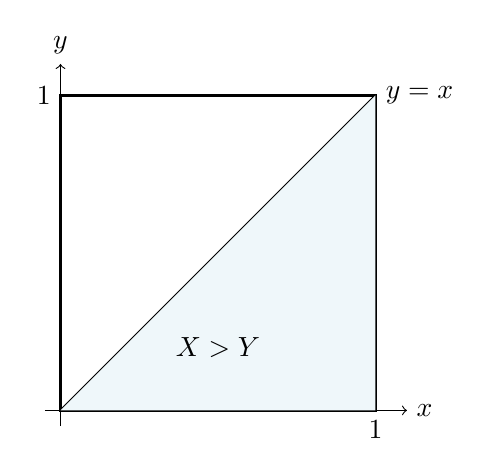
\begin{tikzpicture}[scale=4]
    % Axes
    \draw[->] (-0.05,0) -- (1.1,0) node[right] {$x$};
    \draw[->] (0,-0.05) -- (0,1.1) node[above] {$y$};

    % Unit square
    \draw[thick] (0,0) rectangle (1,1);

    % Diagonal y=x
    \draw[thick] (0,0) -- (1,1) node[right] {$y=x$};

    % Shade region y < x (i.e., X > Y)
    \fill[babyblue!20] (0,0) -- (1,0) -- (1,1) -- cycle;

    % Labels
    \node at (0.5,0.2) {$X>Y$};
    \node[below] at (1,0) {$1$};
    \node[left] at (0,1) {$1$};
\end{tikzpicture}
\end{center}

\textbf{(d) Find \(P(X=Y)\):}

\[
P(X=Y)=\int_0^1 \int_y^y \frac{12}{7}(x^2+xy)\,dx\,dy=0
\]

(Probability along a line is zero for continuous random variables.)

\medskip


\textbf{Example:}

Let the joint PDF be
\[
f(x,y)=
\begin{cases}
e^{-y}, & 0<x<y<\infty \\
0, & \text{otherwise}
\end{cases}
\]

We want to compute
\[
P(X+Y \ge 1).
\]

The support of the joint PDF is the region \(0<x<y\), which lies above the line \(y=x\) in the first quadrant.

The boundary of the event \(X+Y \ge 1\) is the line \(x+y=1\).

Rather than integrating over the unbounded region \(X+Y \ge 1\), we compute the complement:
\[
P(X+Y \ge 1)=1-P(X+Y<1).
\]

The region \(X+Y<1\) that lies within the support is bounded by:
\[
0 \le x \le \tfrac12, \qquad x \le y \le 1-x.
\]

Therefore,
\[
P(X+Y \ge 1)
=
1-\int_0^{1/2}\int_x^{1-x} e^{-y}\,dy\,dx
=
2e^{-1/2}-e^{-1}.
\]

\begin{center}
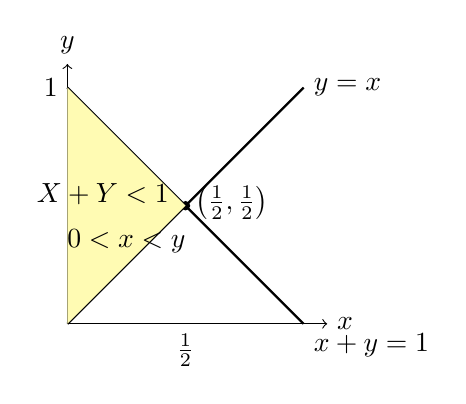
\begin{tikzpicture}[scale=3]

% Axes
\draw[->] (0,0) -- (1.1,0) node[right] {$x$};
\draw[->] (0,0) -- (0,1.1) node[above] {$y$};

% Lines
\draw[thick] (0,0) -- (1,1) node[right] {$y=x$};
\draw[thick] (0,1) -- (1,0) node[below right] {$x+y=1$};

% Intersection point
\fill (0.5,0.5) circle (0.02);
\node[above right] at (0.5,0.4) {$\left(\tfrac12,\tfrac12\right)$};

% Shaded region: x < y < 1-x
\fill[yellow!30] 
(0,0) -- (0.5,0.5) -- (0,1) -- cycle;

% Labels
\node at (0.15,0.55) {$X+Y<1$};
\node at (0.25,0.35) {$0<x<y$};

% Ticks
\node[below] at (0.5,0) {$\tfrac12$};
\node[left] at (0,1) {$1$};

\end{tikzpicture}
\end{center}

\subsection*{Marginal and Conditional PDFs}

\textbf{Def:}  
The \underline{marginal PDFs} of \(X\) and \(Y\) are defined as

\[
g_X(x)=\int_{-\infty}^{\infty} f(x,y)\,dy,
\qquad
h_Y(y)=\int_{-\infty}^{\infty} f(x,y)\,dx
\]

\textbf{Example (continued):}

\[
f(x,y)=
\begin{cases}
\displaystyle \frac{12}{7}(x^2+xy), & 0\le x\le1,\;0\le y\le1 \\
0, & \text{otherwise}
\end{cases}
\]

\textbf{Marginal PDF of \(X\):}
\[
g_X(x)=\int_0^1 \frac{12}{7}(x^2+xy)\,dy
= \frac{12}{7}\left(x^2+\frac{x}{2}\right),
\qquad 0\le x\le1
\]

\textbf{Marginal PDF of \(Y\):}
\[
h_Y(y)=\int_0^1 \frac{12}{7}(x^2+xy)\,dx
= \frac{12}{7}\left(\frac{1}{3}+ \frac{y}{2}\right),
\qquad 0\le y\le1
\]

\textbf{Conditional PDF of \(Y\) given \(X=x\):}

\[
f(y|x)=\frac{f(x,y)}{g(x)}
=\frac{\frac{12}{7}(x^2+xy)}{\frac{12}{7}\left(x^2+\frac{x}{2}\right)},
\qquad 0\le y\le1,\; 0<x\le1
\]

\textbf{Why the bounds are } \(0<x\le1\) \textbf{and not } \(0\le x\le1\):

The marginal PDF
\[
g(x)=\frac{12}{7}\left(x^2+\frac{x}{2}\right)
\]
satisfies \(g(0)=0\).  

Since the conditional PDF is defined as
\[
f_{Y|X}(y|x)=\frac{f(x,y)}{g(x)},
\]
it is \textbf{undefined at \(x=0\)} due to division by zero.

Therefore, the conditional density is only defined for values of \(x\) such that
\[
g(x)>0 \;\Rightarrow\; 0<x\le1.
\]

\textbf{Key takeaway:}  
The bounds of a conditional PDF exclude points where the conditioning density is zero.

\subsection*{Statistical Independence}

\textbf{Def:}  
Random variables \(X\) and \(Y\) (discrete or continuous) are \underline{statistically independent} if and only if

\[
f(x,y)=g(x)\,h(y)
\quad \text{for all } (x,y) \text{ in their range}
\]

\textbf{Consequences:}
\begin{itemize}
    \item \(f(x|y)=g(x)\)
    \item \(f(y|x)=h(y)\)
\end{itemize}


\subsection*{Recall Example: Pen Refills}

Two refills are selected at random and without replacement from a box containing:
\begin{itemize}
    \item 3 blue refills
    \item 2 red refills
    \item 3 green refills
\end{itemize}

Define the random variables
\[
X=\text{number of blue refills selected},\qquad
Y=\text{number of red refills selected}.
\]
Total outcomes:
\[
\binom{8}{2}=28.
\]

\subsection*{Joint PMF Table}

For each pair \((x,y)\),
\[
f(x,y)=\frac{\text{number of favorable outcomes}}{28}.
\]

\begin{center}
\renewcommand{\arraystretch}{2.2}
\begin{tabular}{c|ccc|c}
$X \backslash Y$ & 0 & 1 & 2 & \cellcolor{babyblue!12}$g(x)=P(X=x)$ \\ \hline
0 &
$\dfrac{3}{28}$ &
$\dfrac{3}{14}$ &
$\dfrac{1}{28}$ &
\cellcolor{babyblue!12}$\dfrac{5}{14}$
\\
1 &
$\dfrac{9}{28}$ &
$\dfrac{3}{14}$ &
$0$ &
\cellcolor{babyblue!12}$\dfrac{15}{28}$
\\
2 &
$\dfrac{3}{28}$ &
$0$ &
$0$ &
\cellcolor{babyblue!12}$\dfrac{3}{28}$
\\ \hline
\cellcolor{pink!18}$h(y)=P(Y=y)$ &
\cellcolor{pink!18}$\dfrac{15}{28}$ &
\cellcolor{pink!18}$\dfrac{3}{7}$ &
\cellcolor{pink!18}$\dfrac{1}{28}$ &
\cellcolor{pink!18}$1$
\end{tabular}
\end{center}

\textbf{Marginals:}
\(g(x)=P(X=x)\) is the \underline{marginal PMF of \(X\)} and is given by the \textbf{row totals}.  
\(h(y)=P(Y=y)\) is the \underline{marginal PMF of \(Y\)} and is given by the \textbf{column totals}.

\[
g(0)=\frac{5}{14},\quad g(1)=\frac{15}{28},\quad g(2)=\frac{3}{28}
\]
\[
h(0)=\frac{15}{28},\quad h(1)=\frac{3}{7},\quad h(2)=\frac{1}{28}
\]

\textbf{Independence check:}  
If \(X\) and \(Y\) were \underline{statistically independent}, then \(f(x,y)=g(x)h(y)\) for all \((x,y)\).  
Check \((x,y)=(0,1)\):
\[
f(0,1)=\frac{3}{14},\qquad g(0)h(1)=\left(\frac{5}{14}\right)\left(\frac{3}{7}\right)=\frac{15}{98}
\]
\[
\frac{3}{14}\ne \frac{15}{98}\quad \Rightarrow \quad X \text{ and } Y \text{ are \underline{not independent}.}
\]

\subsection*{Example: Independence via Factorization (Discrete Case)}

Let \(X\) and \(Y\) be \underline{discrete random variables} whose values in the nonnegative integers.

Suppose the joint PMF is
\[
f(x,y)=\frac{1}{x!\,y!}\lambda^x \mu^ye^{-(\lambda+\mu)},
\qquad x,y=0,1,2,\ldots
\]


\textbf{Factorization:}

We can write
\[
f(x,y)=\left(\frac{\lambda^x e^{-\lambda}}{x!}\right)
       \left(\frac{\mu^y e^{-\mu}}{y!}\right)
       = g(x)\,h(y)
\]

\textbf{Marginal PMF of \(X\):}

\[
g(x)=\sum_{y=0}^{\infty} f(x,y)
= \sum_{y=0}^{\infty} \frac{1}{x!\,y!}\,\lambda^x \mu^y\,e^{-(\lambda+\mu)}
\]

Factor out terms that do not depend on \(y\):

\[
g(x)=\frac{1}{x!}\,\lambda^x e^{-(\lambda+\mu)}
\sum_{y=0}^{\infty} \frac{\mu^y}{y!}
\]

Using \(\displaystyle \sum_{y=0}^{\infty}\frac{\mu^y}{y!}=e^{\mu}\):

\[
g(x)=\frac{1}{x!}\,\lambda^x e^{-(\lambda+\mu)} e^{\mu}
=\frac{1}{x!}\,\lambda^x e^{-\lambda},
\qquad x=0,1,2,\ldots
\]

\medskip

\textbf{Marginal PMF of \(Y\):}

\[
h(y)=\sum_{x=0}^{\infty} f(x,y)
= \sum_{x=0}^{\infty} \frac{1}{x!\,y!}\,\lambda^x \mu^y\,e^{-(\lambda+\mu)}
\]

Factor out terms that do not depend on \(x\):

\[
h(y)=\frac{1}{y!}\,\mu^y e^{-(\lambda+\mu)}
\sum_{x=0}^{\infty} \frac{\lambda^x}{x!}
\]

Using \(\displaystyle \sum_{x=0}^{\infty}\frac{\lambda^x}{x!}=e^{\lambda}\):

\[
h(y)=\frac{1}{y!}\,\mu^y e^{-(\lambda+\mu)} e^{\lambda}
=\frac{1}{y!}\,\mu^y e^{-\mu},
\qquad y=0,1,2,\ldots
\]

\textbf{Conclusion:}

Since the joint PMF can be written as
\[
f(x,y)=g(x)\,h(y)
\]
for all \(x,y\), the random variables \(X\) and \(Y\) are \underline{statistically independent}. \(\checkmark\)

\textbf{Important notes:}
\begin{itemize}
    \item Factorization of the joint PMF is \textbf{sufficient} to prove independence.
    \item The constant terms (such as \(e^{-\lambda}\), \(e^{-\mu}\)) must be included to obtain the \textbf{correct marginals}.
    \item  Independence requires that every combination of values with positive marginal probability also has positive joint probability.
\\This means that if \(X=x\) is possible and \(Y=y\) is possible, then the pair \((X=x,Y=y)\) must also be possible.

\[
\{(x,y): f(x,y)>0\}
=
\{x: g(x)>0\}\times\{y: h(y)>0\}.
\]

This means that every value of \(X\) with positive marginal probability can occur with every value of \(Y\) with positive marginal probability.

\end{itemize}

\section*{Jan 30}

\subsection*{Joint distribution}  
Describes probabilities involving two random variables \(X\) and \(Y\).

\begin{itemize}
  \item Discrete:
  \[
  f(X,Y)=P(X=x,Y=y)
  \]
  \item Continuous: joint PDF \(f(X,Y)\)
\end{itemize}

\subsection*{Marginal distribution}  
Obtained by eliminating the other variable.

\begin{itemize}
  \item
  \[
  f(X)=\sum_y f(X,Y), \qquad
  f(Y)=\sum_x f(X,Y)
  \]
  \item
  \[
  f(X)=\int_{-\infty}^{\infty} f(X,Y)\,dy, \qquad
  f(Y)=\int_{-\infty}^{\infty} f(X,Y)\,dx
  \]
\end{itemize}

\subsection*{Joint PDF validity}  
A function \(f(X,Y)\) is a valid joint PDF if:

\begin{itemize}
  \item \(f(X,Y)\ge0\)
  \item
  \[
  \int_{-\infty}^{\infty}\int_{-\infty}^{\infty} f(X,Y)\,dx\,dy=1
  \]
\end{itemize}

\textbf{Example (valid joint PDF):}
\[
f(X,Y)=
\begin{cases}
\dfrac{12}{7}(x^2+xy), & 0\le x\le1,\;0\le y\le1,\\
0, & \text{otherwise}
\end{cases}
\]

\subsection*{Geometric interpretation}  
Probabilities correspond to the \textbf{volume under the surface} \(f(X,Y)\) over a region.

\subsection*{Conditional PDF}  
Distribution of one variable given the other.

\begin{itemize}
  \item
  \[
  f(Y\mid X)=\frac{f(X,Y)}{f(X)}, \quad f(X)>0
  \]
\end{itemize}


\subsection*{Statistical Independence}
\label{sec:independence}

\textbf{Definition:}  
Random variables \(X\) and \(Y\) are \underline{statistically independent} if
\[
f(X,Y)=f(X)f(Y)
\]

This means knowing the value of one variable gives no information about the other.

\subsection*{Support and Independence}

\textbf{Support:}  
The support of a joint distribution is the set
\[
\{(x,y): f(X,Y)>0\}
\]

\textbf{Key idea:}  
If \(X\) and \(Y\) are independent, the support must factor as
\[
\{x:f(X)>0\}\times\{y:f(Y)>0\}
\]

That is, every allowed value of \(X\) can occur with every allowed value of \(Y\).
\subsection*{Example: Non-Independent Random Variables}

\[
f(X,Y)=
\begin{cases}
4(x+y^2), & xy>0,\;x+y\le1,\\
0, & \text{otherwise}
\end{cases}
\]

The condition \(x+y\le1\) links \(x\) and \(y\), so the support does not factor.

\[
\Rightarrow X \text{ and } Y \text{ are not independent}
\]

\textbf{Why this implies dependence (key intuition):}

Pick a value of \(X\) that is allowed:
\[
x=0.8 \quad (\text{positive and } <1)
\]

Pick a value of \(Y\) that is allowed:
\[
y=0.8 \quad (\text{positive and } <1)
\]

Individually, both values are valid.  
But together:
\[
x+y=0.8+0.8=1.6>1
\]

This violates the condition \(x+y\le1\), so the pair \((0.8,0.8)\) is impossible.

\medskip

\textbf{Conclusion:}  
Knowing the value of \(X\) restricts which values \(Y\) can take.  
Therefore, \(X\) and \(Y\) are \underline{not independent}.


\subsection*{Independent Random Variables}

If random variables are independent, joint probabilities factor.

\textbf{Example:}  
Let \(X_1,X_2,X_3\) be independent with
\[
f(X)=e^{-x}, \quad x>0
\]

Then
\[
f(X_1,X_2,X_3)=e^{-x_1}e^{-x_2}e^{-x_3}
\]

\[
P(X_1<2,\;1<X_2<3,\;X_3>2)
=
(1-e^{-2})(e^{-1}-e^{-3})e^{-2}
\]
\textbf{Explanation (why this works):}

Since \(X_1,X_2,X_3\) are \underline{independent}, the joint probability factors:
\[
P(X_1<2,\;1<X_2<3,\;X_3>2)
=
P(X_1<2)\,P(1<X_2<3)\,P(X_3>2)
\]

For an exponential random variable with
\[
f(X)=e^{-x}, \quad x>0,
\]
we have:
\[
P(X<a)=1-e^{-a}, \qquad P(X>a)=e^{-a}
\]

Thus,
\[
P(X_1<2)=1-e^{-2}
\]
\[
P(1<X_2<3)=P(X_2<3)-P(X_2<1)=e^{-1}-e^{-3}
\]
\[
P(X_3>2)=e^{-2}
\]

Multiplying gives:
\[
(1-e^{-2})(e^{-1}-e^{-3})e^{-2}
\]



\subsection*{Mutual Independence and Modeling Assumptions}

\textbf{Mutual independence:}  
Random variables \(X_1,\ldots,X_n\) are mutually independent if
\[
f(X_1,\ldots,X_n)=\prod_{i=1}^n f(X_i)
\]

Pairwise independence does \textbf{not} imply mutual independence.

\medskip

\textbf{Independent selection:}
Selections are independent if:
\begin{itemize}
  \item each selection is random,
  \item distributions are identical,
  \item outcomes do not affect future selections.
\end{itemize}

Sampling without replacement generally produces \underline{dependent} variables.

\section*{Chapter 4}

\subsection*{Motivation}

\textbf{Example:}  
If you roll a fair die repeatedly, what \textit{average value} do you expect in the long run?

\medskip
This motivates the idea of \underline{expectation}: a theoretical long-run average.

\subsection*{Expectation (Expected Value)}

\textbf{Def:}  
For a random variable \(X\), the \underline{expectation} (or \underline{expected value} or \underline{mean}) is the long-run average value of \(X\).

\medskip

\textbf{Discrete random variable:}
\[
\boxed{
\mu = E(X)=\sum_x x\,f(X)
}
\]

\textbf{Continuous random variable:}
\[
\boxed{
\mu = E(X)=\int_{-\infty}^{\infty} x\,f(X)\,dx
}
\]

\medskip
\textbf{Interpretation:}  
Expectation is a \underline{weighted average}, where values of \(X\) are weighted by how likely they are.

\subsection*{Example: Fair Die}

Let \(X\) be the outcome when a fair die is rolled.

\[
E(X)=\sum_{x=1}^6 x\cdot\frac{1}{6}
\]

\[
E(X)=\frac{1+2+3+4+5+6}{6}=3.5
\]

\medskip
Even though 3.5 is not a possible outcome, it represents the \underline{long-run average}.

\subsection*{Example: Number of Messages per Hour}

Let \(X\) be the number of messages sent per hour, with PMF:

\[
\begin{array}{c|cccccc}
x & 10 & 11 & 12 & 13 & 14 & 15 \\ \hline
f(X) & 0.08 & 0.15 & 0.30 & 0.20 & 0.20 & 0.07
\end{array}
\]

\textbf{Check:}
\[
\sum f(X)=1
\]

\textbf{Expected value:}
\[
\begin{aligned}
E(X)
&=10(0.08)+11(0.15)+12(0.30)+13(0.20)+14(0.20)+15(0.07) \\
&=12.5
\end{aligned}
\]

\medskip
This means that over many hours, the average number of messages per hour is about 12.5.

\subsection*{PMF Visualization}

\begin{center}
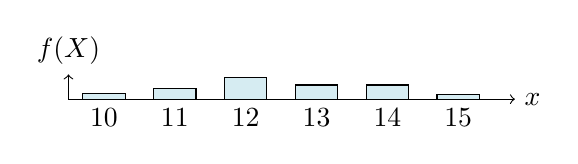
\begin{tikzpicture}[scale=0.9]

% Axes
\draw[->] (9.5,0) -- (15.8,0) node[right] {$x$};
\draw[->] (9.5,0) -- (9.5,0.35) node[above] {$f(X)$};

% Bars
\foreach \x/\p in {10/0.08,11/0.15,12/0.30,13/0.20,14/0.20,15/0.07}
{
    \draw[fill=babyblue!50] (\x-0.3,0) rectangle (\x+0.3,\p);
}

% Labels
\node[below] at (10,0) {10};
\node[below] at (11,0) {11};
\node[below] at (12,0) {12};
\node[below] at (13,0) {13};
\node[below] at (14,0) {14};
\node[below] at (15,0) {15};

\end{tikzpicture}
\end{center}

\subsection*{Example: Deal or No Deal}

Consider a game with two possible outcomes:
\begin{itemize}
    \item \$1 with probability \(1/2\)
    \item \$10{,}000 with probability \(1/2\)
\end{itemize}

\textbf{Expected value:}
\[
E(X)=\frac{1}{2}(1)+\frac{1}{2}(10{,}000)=5000.5
\]

\medskip
\textbf{Key idea:}  
The expected value is the \underline{average payout in the long run}, not the most likely outcome.

\subsection*{Example: Continuous RV (Device Lifetime)}

Let \(X\) be a random variable that denotes the lifetime (in hours) of a certain device, with PDF
\[
f(X)=
\begin{cases}
\dfrac{20000}{x^3}, & x>100,\\
0, & \text{otherwise.}
\end{cases}
\]

\textbf{Check (valid PDF):}
\[
\int_{-\infty}^{\infty} f(X)\,dx
=
\int_{100}^{\infty} \frac{20000}{x^3}\,dx
=
20000\left[\frac{-1}{2x^2}\right]_{100}^{\infty}
=
1
\]

\textbf{Expected lifetime:}
\[
E(X)=\int_{100}^{\infty} x\frac{20000}{x^3}\,dx
=
\int_{100}^{\infty}\frac{20000}{x^2}\,dx
=
20000\left[\frac{-1}{x}\right]_{100}^{\infty}
=
200
\]

So we expect this type of device to last on average \(\boxed{200}\) hours.

\subsection*{Example: Discrete RV and Transformation}

Let \(X\) be a discrete random variable with PMF:

\[
\begin{array}{c|cccc}
x & -1 & 0 & 1 & 2 \\ \hline
f(X) & 0.3 & 0.2 & 0.3 & 0.2
\end{array}
\]

Define a new random variable as a \underline{transformation} of \(X\):
\[
g(X)=X^2
\]

\textbf{Possible values of \(g(X)\):}
\[
g(-1)=1,\quad g(0)=0,\quad g(1)=1,\quad g(2)=4
\]
So \(g(X)\) can take values \(\{0,1,4\}\).

\textbf{Distribution of \(g(X)\):}
\[
P(g(X)=0)=P(X=0)=0.2
\]
\[
P(g(X)=1)=P(X=-1)+P(X=1)=0.3+0.3=0.6
\]
\[
P(g(X)=4)=P(X=2)=0.2
\]

\[
\begin{array}{c|ccc}
g(X) & 0 & 1 & 4 \\ \hline
P(g(X)) & 0.2 & 0.6 & 0.2
\end{array}
\]

This is called a \underline{transformation} of a random variable.

\textbf{Expected value of the transformed RV:}
\[
\boxed{
E(g(X))=E(X^2)=\sum_x x^2 f(X)=\sum_x g(x)\,f(X)
}
\]

Numerically:
\[
E(X^2)=0^2(0.2)+(-1)^2(0.3)+(1)^2(0.3)+(2)^2(0.2)
=0+0.3+0.3+0.8=1.4
\]

\begin{center}
\begin{tcolorbox}[
    colback=softpink!5,
    colframe=softpink!70!black,
    coltitle=black,
    colbacktitle=softpink,
    title=\textbf{Expected Value of a Function of a RV},
    boxrule=0.8pt,
    arc=6pt,
    width=0.9\textwidth
]
Let \(X\) be a random variable with distribution \(f(X)\). The expected value of the random variable \(g(X)\) is

\[
\boxed{
E(g(X))=
\begin{cases}
\sum_x g(x)\,f(X), & \text{if \(X\) is discrete}\\[6pt]
\int_{-\infty}^{\infty} g(x)\,f(X)\,dx, & \text{if \(X\) is continuous}
\end{cases}
}
\]
\end{tcolorbox}
\end{center}

\subsection*{Example: Chip Game (Expected Winnings)}

A bowl contains 5 chips:
\begin{itemize}
  \item 3 chips are worth \$1 each
  \item 2 chips are worth \$4 each
\end{itemize}
A player draws 2 chips at random (without replacement) and is paid the sum.

\medskip
Let \(X\) be the number of \$1 chips drawn. Then
\[
X\in\{0,1,2\}.
\]

\textbf{PMF of \(X\):} (hypergeometric)
\[
f(X)=
\begin{cases}
\dfrac{\binom{3}{x}\binom{2}{2-x}}{\binom{5}{2}}, & x=0,1,2,\\[8pt]
0, & \text{otherwise.}
\end{cases}
\]

\textbf{Define payout as a function of \(X\):}  
If you draw \(x\) one-dollar chips, then you draw \(2-x\) four-dollar chips, so the payout is
\[
g(x)=1(x)+4(2-x)=8-3x.
\]
So the payout random variable is \(g(X)=8-3X\).

\textbf{Expected payout:}
\[
E(g(X))=\sum_{x=0}^{2} g(x)\,f(X)
\]

Compute \(f(X)\) values:
\[
f(0)=\frac{\binom{3}{0}\binom{2}{2}}{\binom{5}{2}}=\frac{1}{10},\quad
f(1)=\frac{\binom{3}{1}\binom{2}{1}}{\binom{5}{2}}=\frac{6}{10},\quad
f(2)=\frac{\binom{3}{2}\binom{2}{0}}{\binom{5}{2}}=\frac{3}{10}.
\]

Then
\[
E(g(X))=\sum_{x=0}^{2} (8-3x)\,f(X)
=
(8)\left(\frac{1}{10}\right)
+(5)\left(\frac{6}{10}\right)
+(2)\left(\frac{3}{10}\right)
=4.4
\]

\textbf{Decision:}  
If it costs \$4.75 to play, your expected profit is
\[
E(\text{profit})=E(g(X)) - 4.75 = 4.4-4.75=-0.35
\]
So in the long run, you lose about \(\boxed{\$0.35}\) per game on average, so you should \underline{not} play.

\subsection*{Notation: \(g(X)\) vs. \(g(x)\)}

\begin{itemize}
  \item \(X\) is a \underline{random variable}; \(x\) is a specific value it can take.
  \item \(g(X)\) is a \underline{random variable}.
  \item \(g(x)\) is a \underline{number}.
\end{itemize}

\medskip

\textbf{Key rule:}
\[
\boxed{
E(g(X))=\sum_x g(x)\,f(X)
}
\]

Expectation averages the numerical values \(g(x)\), weighted by their probabilities.

\medskip

\textbf{Exam rule:}  
\[
\boxed{g(X)\text{ is random variable, } g(x)\text{ is a number.}}
\]

\end{document}
